% Pages in Thesis should have one of standard U.S. Paper Sizes
% U.S Letter Paper (8.5 x 11) is used.
% Body should be either 11 pt or 12 pt type.
\documentclass[12pt, letterpaper]{thesis}

\usepackage{hyperref}
%\usepackage[sorting=debug]{biblatex}
\usepackage[style=numeric,giveninits]{biblatex}
\usepackage{afterpage}
\addbibresource{references.bib}
% For mathematical symbols such as degree
\usepackage{textcomp}
\usepackage{gensymb}
\usepackage{booktabs}
\usepackage{amsthm}
\usepackage{pdflscape}
\usepackage{rotating}
\usepackage{mathpazo}
\usepackage{longtable}
\usepackage[linesnumbered,ruled,vlined]{algorithm2e}

\date{}
\begin{document}

% Front Matter
% Except for the "Abstract" page, every page of thesis must be assigned a
% page number. Placement of consistent page numbers is necessary, and they
% must either be at center, or at the top-right corner.
% Page numbering should be roman numerals for the front matter, and numbered
% for main text.
% Hide page numbers for this page.
\thispagestyle{empty}
\newgeometry{top=1.75in, left=1.5in, right=1in, bottom=1in}
\begin{center}
    EXPLORING THE LIMITS OF ZERO-SHOT LEARNING - HOW LOW CAN YOU GO ?
    
    by
    
    HEMANTH DANDU
    
    (Under the Direction of Suchendra Bhandarkar)
    
    ABSTRACT
\end{center}
Zero-shot learning aims to classify input data into categories with zero training examples. The classification is performed by inferring unseen categories using visual data of seen categories and their relationships with unseen categories. Relationships are determined by using auxiliary data pertaining to categories such as attributes and semantics. Standard zero-shot learning techniques use a large number of seen categories to predict very few unseen categories while maintaining unified data splits and evaluation metrics. This has enabled the research community to advance notably towards formulating a standard benchmark zero-shot learning algorithm. However, the most substantial impact of zero-shot learning lies in enabling the prediction of a large number of unseen categories from very few seen categories within a specific domain. This permits the collection of training data for only a few previously seen categories, thereby mitigating the training data collection process significantly. In this thesis, we focus on the difficult problem of predicting a large number of unseen object categories from very few previously seen categories. We propose a framework that enables us to examine the limits of inferring several unseen object categories from very few previously seen object categories, i.e., the limits of zero-shot learning. In particular, we examine the functional dependence of the classification accuracy of unseen object classes on the number of previously seen classes. We also determine the minimum number of previously seen classes required to achieve pre-specified classification accuracy for the unseen classes on three standard zero-shot learning data sets, i.e., AWA2, CUB and SUN. Additionally, we compare the proposed framework with a prominent zero-shot learning technique on the aforementioned data sets and find that we achieve 21\% higher accuracy on the AWA2 data set, 6\% higher accuracy on the CUB data set, and comparable performance on the SUN data set while providing valuable insights into the unseen class inference process.

%\vspace{2\baselineskip}
\noindent
INDEX WORDS: machine learning, image classification, zero-shot learning, transfer learning

\newpage
\pagenumbering{roman}
% Hide page numbers for this page.
\thispagestyle{empty}
\newgeometry{top=1.75in, left=1.5in, right=1in, bottom=1in}
\begin{center}
    AN EXPLORATION OF MACHINE LEARNING BASED DAY-AHEAD SOLAR IRRADIANCE FORECASTING METHODOLOGIES
    
    \vspace*{2\baselineskip}
    by

    \vspace*{2\baselineskip}
    AASHISH YADAVALLY
    
    B.Tech., Indian Institute of Information Technology Vadodara, INDIA, 2018
    \vspace*{4\baselineskip}

    A Thesis Submitted to the Graduate Faculty of The University of Georgia
    in Partial Fulfillment of the Requirements for the Degree
    \vspace*{3\baselineskip}

    MASTER OF SCIENCE
    \vspace*{3\baselineskip}

    ATHENS, GEORGIA
    
    2020
\end{center}

\newpage
% Hide page numbers for this page.
\thispagestyle{empty}

\begin{center}
    \vspace*{18\baselineskip}
    \textcopyright \hspace{0.05cm} 2020
    
    Hemanth Dandu
    
    All Rights Reserved
\end{center}

\newpage
% Hide page numbers for this page.
\thispagestyle{empty}
\newgeometry{top=1.75in, left=1.5in, right=1in, bottom=1in}
\begin{center}
    EXPLORING THE LIMITS OF ZERO-SHOT LEARNING - HOW LOW CAN YOU GO ?
    
    \vspace*{1\baselineskip}
    by
    \vspace*{1\baselineskip}

    HEMANTH DANDU
\end{center}

\vspace*{6\baselineskip}

\iffalse
\begin{flushright}
Major Professor: $\hskip 0.5em$ Suchendra Bhandarkar
\vspace{\baselineskip}

Committee: \hspace{12pt} $\hskip 2.25em$ Khaled Rasheed \hspace{12pt}\\
Frederick Maier  \\
Karan Sharma  
\end{flushright}
\fi

\begin{flushright}
  \begin{tabular}{ll}
 Major Professor: &Suchendra Bhandarkar \\  [10pt]
    Committee: &Khaled Rasheed \\
    &Frederick Maier \\
    &Karan Sharma \\
  \end{tabular}
\end{flushright}
\vspace*{3cm}


\vspace{3\baselineskip}
\noindent
Electronic Version Approved:\\
Ron Walcott\\
Dean of the Graduate School\\
The University of Georgia\\
December 2020
\newpage
\chapter{1}{Acknowledgements}{Acknowledgements}
\par I would like to thank all my committee members for their time and the numerous suggestions they provided throughout my research. In particular, I would like to thank Dr. Maier for his guidance, constant encouragement and motivation to keep me going. I owe a great debt to Zachary Jones and Chris Barrick who facilitated my introduction into the project, and whose contributions laid the foundation for my work. I am thankful to my friends and family who kept me sane during these unprecedented times, where the whole world has come to a standstill due to COVID-19. I would like to thank everyone at the \textit{Institute for Artificial Intelligence} who presented me with an opportunity to be a part of this project. I would also like to thank Ms. Tino, whose assistance with the administrative tasks at the university made my life incredibly easy.

\newpage
% Print Table of Contents
\listofchapter
\newpage
% Add List of Tables chapter
\listoftables
% Add List of Tables chapter to Table of Contents
\addcontentsline{chl}{chapter}{~LIST OF TABLES}
\newpage
% Add List of Figures chapter
\listoffigures
% Add List of Figures chapter to Table of Contents
\addcontentsline{chl}{chapter}{~LIST OF FIGURES}
\newpage

\theoremstyle{definition}
\newtheorem{definition}{Definition}[chapter]

% Chapters in Thesis
% Chapter 1: Introduction
\pagenumbering{arabic}
\chapter{}{Introduction}{Introduction}

Advances in deep neural networks have empowered machines to achieve human level classification performance on object recognition tasks. Very powerful and robust visual classifier frameworks have been developed, and will no doubt keep improving. In typical object recognition tasks, it is necessary to establish a certain number of predetermined object categories so that classification accuracy can be improved by collecting as many training image samples as possible for each object category. Many problem domains are faced with a large and growing number of object categories. As a consequence, it is becoming increasingly difficult to collect and annotate training data for each object category. Moreover, these images need to capture different aspects of the objects under various imaging conditions to account for the natural variance in appearance for each object category. The problem thus lies in collecting and annotating training data in an efficient and reliable manner for a wide variety of object categories. In addition, trained classifiers can only classify observed object instances into the classes or categories covered by the training data; they lack the ability to deal with previously unseen classes. To address this issue, zero-shot learning (ZSL) techniques have been proposed in the research literature. ZSL frameworks are designed to  tackle the problem of learning classifiers when no explicit visual training examples are provided.

\par
\medskip

Human beings perform ZSL naturally, enabling recognition of at least 30,000 object classes~\cite{humanimageunderstanding}. When faced with a new unfamiliar object, we are, after a while, able to state what it resembles: "A New York City hot dog cart, with the large block being the central food storage and cooking area, the rounded part underneath as a wheel, the large arc on the right as a handle, the funnel as an orange juice squeezer and the various vertical pipes as vents or umbrella supports." It is not a good cart, but we can see how it might be related to one~\cite{humanimageunderstanding}. For humans, it is as easy as recognizing a 10-letter word with 3 wrong letters. However, in the case of machines, we need a vast number of training images for each type of cart to learn to adapt to the naturally occurring variations in cart appearances. In humans, the ability to understand natural variations comes from our existing and ever evolving language knowledge base, which enables us to connect unseen categories with seen categories using high-level descriptions.

\par
\medskip

To emulate the ZSL process in machines, previously unseen object categories are recognized by leveraging auxiliary information related to categories. Auxiliary information are derived from external data sources such Wikipedia, WordNet~\cite{wordnet} etc. which make it analogous to the human (natural language) knowledge base. As the auxiliary inputs usually carry semantic information, they constitute a \textit{semantic space}. A typical source of semantic information used in ZSL is \textit{attribute spaces}. Attribute spaces are semantic spaces that are engineered manually for each domain or data set. Attributes are a list of terms that describe various properties of each object class or category. For example, an attribute could be \textit{hair color} with values "black", "brown", "white" etc. The attributes can be either discrete or continuous. Label-embedding spaces are also often used as a source of semantic information, where the word/label representations are obtained by employing information retrieval techniques on large digital text corpora. Examples of widely used label-embedding models include Word2Vec~\cite{w2v}, GloVe~\cite{glove}, and FastText~\cite{fasttext}. Hierarchical information is another source of semantic information that can be derived from a pre-existing ontology such as WordNet \cite{wordnet}. All sources of auxiliary information when combined together comprise the semantic space.

\par
\medskip

In typical ZSL frameworks, a set of previously observed classes is used to train the visual classifier. These classes are termed as \textit{seen classes}. The framework is then evaluated on another set of previously not observed classes termed as \textit{unseen classes}. While training, the classifier has access to auxiliary information of both the seen and unseen classes. A formal definition of the ZSL task is provided in Definition~\ref{def:zsl}. 
Conventional ZSL is restrictive in its formulation since it assumes that the input images at the time of  prediction or inference can only come from the unseen classes. In contrast, generalized ZSL addresses the more general setting where the input images at the time of  prediction or inference can come from both, the seen and unseen classes~\cite{gen-zsl}. Generalized ZSL is formally defined in Definition \ref{def:gzsl}. 

\par
\medskip

\theoremstyle{definition}
\begin{definition}[Conventional Zero-shot Learning]
\label{def:zsl}
Given labelled training instances $X_s$ belonging to seen classes $Y_s$, zero-shot learning aims to learn a classifier that can classify testing instances $X_u$ belonging to the unseen classes $Y_u$
\end{definition}

\par
\medskip

\theoremstyle{definition}
\begin{definition}[Generalised Zero-shot Learning]
\label{def:gzsl}
Given labelled training instances $X_s$ belonging to seen classes $Y_s$, generalised zero-shot learning aims to learn a classifier that can classify testing instances $X_{u \cup s}$ belonging to the classes $Y_u \cup  Y_s$
\end{definition}

\par
\medskip

Several ZSL frameworks have been proposed in the literature, however, all of these frameworks use a proposed split~\cite{gbu} of standard ZSL data sets~\cite{awa,cub,sun} into seen and unseen classes. This split is formulated in to aid uniform research towards finding a universal ZSL framework that outperforms the existing ones. Altogether, the zero-shot learning problem has been formally framed for each standard data set using specific categories as seen classes and the remaining as unseen classes in a race for attaining maximum classification accuracy. Of the total object categories present in each data set, the number of seen classes has always been significantly higher than the number of unseen classes in most ZSL frameworks. For example, the \textit{Animals-with-Attributes} (AWA2) data set~\cite{awa} has a proposed 40:10 seen:unseen class split, the \textit{Caltech-USCD-Birds} (CUB) data set~\cite{cub} has a 150:50 seen:unseen class split, and the large-scale \textit{Scene Understanding} (SUN) database~\cite{sun} has a 645:72 seen:unseen class split. While this formulation has helped to formulate several benchmark approaches to ZSL tasks, we notice that the original intent of mitigating the data collection process has been skirted at a very early stage. Therefore, we aim to infer larger number of unseen object categories using very few seen object categories. We believe this addresses the original problem of obtaining annotated images to a greater extent. 

\par
\medskip

We propose a new framework that helps us to examine the limits of inferring unseen object categories from very few seen object categories, i.e., test the limits of ZSL. We note the functional dependence of the classification accuracy on the number of previously seen classes across the spectrum of the classes on three widely used object classification data sets~\cite{awa,cub,sun}. An important contribution of the proposed approach is its ability to determine the optimal set of representative classes using which one could infer a large number of previously unseen classes with a pre-specified measure of accuracy. We explore intuitive techniques to select a few seen classes which would enable us to predict a larger number of unseen classes. The proposed approach also aids the training data collection process significantly by identifying the key object categories from which the training data collection process can be initiated and determining which object categories to stop at, based on an expected or pre-specified classification accuracy measure for a specific problem. We evaluate the proposed approach in the generalized ZSL setting, thus making it very practical. We present valuable insights into the inference process for general and specific cases where the proposed approach performs exceptionally well, and also for cases where we fail to infer the correct unseen category. We also compare the proposed approach with the well known Attribute Label Embedding (ALE)~\cite{ale} procedure, which has been shown to perform very well on the aforementioned three standard data sets as published in~\cite{gbu}. In comparison to ALE, we observe that the proposed approach achieves 21\% higher accuracy on the AWA2 data set, 6\% higher accuracy on the CUB data set and comparable performance on the SUN data set. We also establish the minimum number of previously seen classes needed to obtain reasonable (or above average) generalized ZSL performance on the AWA2 data set as 20 seen classes out of a total of 50 classes, on the CUB data set as 80 seen classes out of a total of 200 classes and on the SUN data set as 360 seen classes out of a total of 717 classes.

\par
\medskip

This thesis is organized into six chapters. Chapter 1 introduces the concept of zero-shot learning (ZSL) and summarizes the work done in this thesis. Chapter 2 reviews the related work in ZSL and position our work in the overall ZSL research literature. Chapter 3 describes the various data sets used for experiments carried out in this thesis. Chapter 4 discusses the overall methodology underlying the proposed approach and also explains the finer details about the methods used. Chapter 5 presents the experimental results of the proposed approach on the aforementioned three data sets. Chapter 5 compares the proposed approach with the Attribute Label Embedding (ALE) scheme and shows how well the proposed approach fares in comparison to the widely used ALE-based ZSL framework. Finally, in Chapter 6, we conclude this thesis and discuss directions for future work.
% Chapter 2: Related Work
\chapter{}{Literature Review}{Literature Review}

Zero-shot learning (ZSL) approaches can be broadly classified into two categories based on the unseen class information the model has during the training process. In the inductive ZSL framework, we have access to to labeled image data from the seen classes as well as auxiliary information (i.e., semantic attributes/descriptions) about both, seen and unseen classes during the training phase. In the transductive ZSL framework, we have access to auxiliary information (i.e., semantic attributes/descriptions) about both, seen and unseen classes during the training phase as in the case of the inductive ZSL framework. The major difference is that in the case of transductive ZSL, we have access to labeled image data from the seen classes \textit{and} unlabeled image data from the unseen classes during the training phase which is a departure from inductive ZSL. Within both frameworks, one can make an distinction based on the type of setting used to evaluate the model during testing. i.e. the conventional ZSL setting and generalized ZSL setting as described in Chapter 1. In this section we review work on both the inductive and transductive ZSL frameworks and place the proposed approach within the ZSL taxonomy.

\par
\medskip

Preliminary work in inductive ZSL uses a two-stage approach to infer unseen class labels. In the first stage, the attributes of an image are predicted. In the next stage, the class label is inferred by searching for the class label with the most similar set of attributes. Lampert et al~\cite{DAP} introduced the Directed Attribute Prediction (DAP) and Indirect Attribute Prediction (IAP) models  which use the aforementioned two-stage approach. In DAP~\cite{DAP}, a probabilistic attribute classifier is first learned. The class posteriors are then computed and class labels predicted via a maximum a posteriori (MAP) estimate. In IAP~\cite{DAP}, a multi-class classifier is first used to predict the class posterior. The probability of each class is then used to compute the attribute posteriors of an image. While the DAP and IAP frameworks have historically been some of the most widely cited ZSL methods in the literature, they suffer from the problem of domain shift~\cite{domainshift} where the intermediate functions learned from the auxiliary information without any adaptation to the target domain introduce an unknown bias.

\par
\medskip

Subsequent ZSL frameworks attempt to learn a compatibility function from image feature space to the semantic or auxiliary space. These frameworks can be further categorized based on the type of compatibility function that they learn. The first set of methods learn linear compatibility functions whereas the next set of methods learn non-linear compatibility functions.

\par
\medskip

\noindent
\textbf{Linear Compatibility.} Attribute Label Embedding (ALE)~\cite{ale} learns a bi-linear compatibility function between the image space and auxiliary space using a weighted approximate ranking objective. ALE improves upon DAP \cite{DAP} significantly since it can use multiple sources of auxiliary information such as word embeddings and class taxonomies. ALE also overcomes the drawbacks of the two-step process used in DAP by directly predicting the class label without the need for an intermediate step. The Deep Visual-Semantic Embedding (DEVISE) model~\cite{devise} also learns a linear mapping between the image space and semantic space and has been shown to perform well on the large-scale ImageNet data set. The Structured Joint Embedding (SJE) scheme~\cite{SJE} uses an unregularized structured SVM to learn the compatibility function coupled with the Stochastic Gradient Descent (SGD) algorithm for optimization. The Embarrassingly Simple Zero-Shot Learning (ESZSL) scheme~\cite{ESZSL} uses an additional regularization term to suppress noise in the auxiliary space. 

\par
\medskip

\noindent
\textbf{Non-Linear Compatibility.}  The Latent Embedding (LATEM) scheme~\cite{LATEM} extends linear compatibility approaches by learning multiple mappings thereby finding a piece-wise linear compatibility function using every image-class pair. LATEM shows improved accuracy over the state-of-art the linear compatibility-based SJE scheme~\cite{SJE}. The Cross-Modal Transfer (CMT) scheme~\cite{CMT} uses a neural network with two hidden layers to learn non-linear projections from image space to Word2Vec~\cite{w2v} space. CMT exploits only information from word embeddings and does not use other sources of auxiliary information such as class attributes used by other methods.
%%% SMB: INCLUDE THE FOLLOWING REFERENCE AND CITATION FOR CMT:
%%% R. Socher, M. Ganjoo, C.D. Manning and A.Y. Ng, Zero-Shot Learning Through Cross-Modal Transfer, Proc. NIPS 2013.  

\par
\medskip

Drawing from linear and non-linear compatibility approaches, hybrid models~\cite{gbu} learn a joint embedding of both the image and semantic features into a combined intermediate space. The Semantic Similarity Embedding (SSE) scheme~\cite{sse} uses a max-margin framework to jointly optimize domain data and semantic data. The Convex Combination of Semantic Embeddings (CONSE) scheme~\cite{conse} is inspired by DEVISE~\cite{devise} and maps images into the semantic embedding space via convex combination of the class label embedding vectors without the need for additional training. Synthesized Classifiers (SYNC) \cite{sync} introduces a set of “phantom” object classes whose coordinates exist in both the semantic space and the model space which are then optimized using labeled data such that the synthesized real object classifiers achieve optimal discriminating performance. Wang et al.~\cite{gcn} use a Graph Convolution Network (GCN) and the GLoVe text embedding model~\cite{glove} to generate a knowledge graph embedding. The knowledge graph embedding exploits both, semantic embeddings and domain relationships to predict the object classifiers. 
%%% SMB: INCLUDE THE FOLLOWING REFERENCE AND CITATION FOR CONSE:
%%% M. Norouzi, T. Mikolov, S. Bengio, Y. Singer, J. Shlens, A. Frome, G.S. Corrado, and J. Dean, Zero-Shot Learning by Convex Combination of Semantic Embeddings, Proc. ICLR, 2014. 

\par
\medskip

Recently, there has been a rise in the use of generative models for ZSL that represent each class as a probability distribution. Generative Framework for Zero-Shot Learning (GFZSL)~\cite{gfzsl} models the class-conditional distributions of seen as well as unseen classes using a multi-variate Gaussian distribution. Generative models such as GFZSL exhibit a significant performance boost in the transductive ZSL setting. The Feature Generating Network (FGN)~\cite{fgn} introduces a novel Generative Adversarial Network (GAN) that synthesizes Convolutional Neural Network (CNN) features conditioned on class-level semantic information, offering a direct shortcut  from a semantic descriptor of a class to a class-conditional feature distribution. The Leveraging the Invariant Side GAN (LisGAN) approach~\cite{LISGAN} generates unseen features from random noise functions which are conditioned by the semantic descriptions. They train a conditional Wasserstein GAN in which the generator synthesizes fake unseen features from noises and the discriminator distinguishes the fake from real via a minimax game. The recent approach based on leveraging the semantic relationships between the seen and unseen object categories termed as LsrGAN~\cite{lsrGAN} performs explicit knowledge transfer by incorporating a novel Semantic Regularized Loss (SR-Loss) function. A Tensorflow-based combination of a Variable Auto-Encoder (VAE) and GAN, termed as TF-vaegan~\cite{tf-vegan}, introduces a feedback loop from a semantic embedding decoder, that iteratively refines the generated features during both the training and feature synthesis stages. The synthesized features together with their corresponding latent embeddings from the decoder are then transformed into discriminative features and exploited during classification to reduce the ambiguities amongst the categories. The TF-vaegan framework~\cite{tf-vegan} is currently regarded as the benchmark in inductive and transductive ZSL settings on the AWA2~\cite{awa}, CUB~\cite{cub}, and SUN~\cite{sun} data sets on the zero-shot learning and generalized zero-shot learning settings. 

\par
\medskip

The proposed framework draws from the two-stage approach used by the DAP and IAP approaches~\cite{DAP} but the problem being addressed is substantially different from the standard ZSL problem that the aforementioned ZSL frameworks are designed for. Note that the proposed approach aims to predict a large number of unseen classes from few seen classes, and consequently, we have far less training data compared to the conventional ZSL settings. Hence, generative-adversarial-based and compatibility learning-based ZSL frameworks which require a lot of training data would be expected to perform poorly in this situation. The proposed ZSL framework represents a first step towards a novel ZSL problem formulation that strives to understand how classification accuracy measures change with change in number and type of seen classes. The proposed framework also allows for selection of an optimal number and type of seen classes based on an expected overall classification accuracy measure which aids in the training data collection process.

\newpage
% Chapter 3: Datasets
\chapter{}{{Data Sets}}{Data Sets}

This chapter describes the three data sets used in the experiments in this thesis. Table \ref{table:data_stats} shows the summary statistics for all three data sets.

\subchapter{Animals with Attributes-2 (AWA2)}
The Animals with Attributes (AWA) data set was originally introduced by Lampert et al.~\cite{DAP}. Since the original images from AWA were not publicly available, Xian et al.~\cite{gbu} enhanced the AWA data set and termed it as Animals with Attributes-2 (AWA2)~\cite{awa}, while retaining the same animal classes and attributes as AWA. AWA2 has a total of 37,322 images compared to 30,475 images in AWA. AWA2 is considered a coarse-grained data set that is medium-scale in terms of images and small-scale in terms of number of classes, i.e. 50 animal classes. The data also provides 85 numeric attribute values for each class. Using the shared attributes, it is possible to transfer information between different classes. The AWA2 data set permits evaluation of the proposed approach in a coarse-grained domain with a small number of classes. A few examples of animal classes in AWA2 are \textit{polar bear}, \textit{zebra}, \textit{otter}, and \textit{tiger}. Figure \ref{image:awa2} shows a few images from the AWA2 data set where the image data was collected from public sources, such as Flickr in 2016. Further information about the data set can be found here \footnote{https://cvml.ist.ac.at/AwA2/}.

\begin{figure}[ht]
\centering
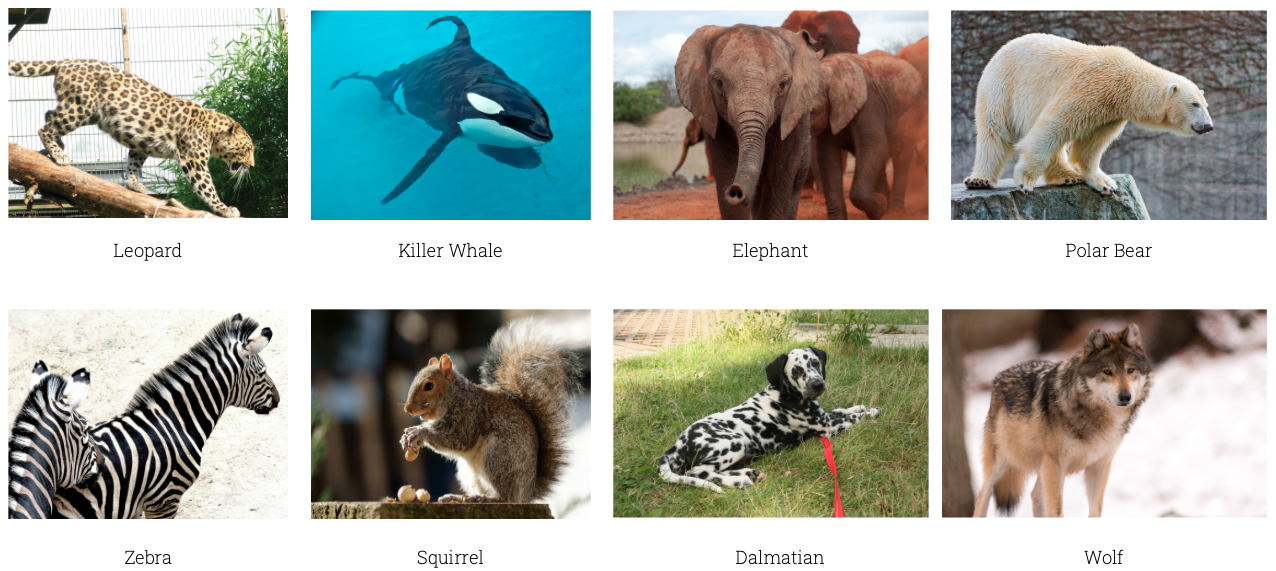
\includegraphics[width=\textwidth]{MS-Thesis-master/figures/awa2_new.png}
\caption{A few labelled images from the Animals with Attributes-2 (AWA2) data set.}
\label{image:awa2}
\end{figure}

\subchapter{Caltech-UCSD Birds (CUB)}

The Caltech-UCSD Birds-200-2011 (CUB) data set~\cite{cub} is an image data set with 11,788 photographs of 200 bird species. Each species is associated with a Wikipedia article and organized by its scientific classification, i.e., (order, family, genus, species). The list of species names was obtained using an online field guide. Each image is annotated with a bounding box, part location, and attribute labels, thereby providing 312 numeric attribute values for each class. CUB is considered a fine-grained data set that is medium-scale in terms of both images and classes. This data set allows evaluation of the proposed approach in a fine-grained domain with a moderate number of classes. A few examples of bird species are \textit{Long tailed Jaeger}, \textit{Blue-winged Warbler}, \textit{American Crow}, \textit{Louisiana Waterthrush}, and \textit{Herring Gull}. Figure~\ref{image:cub} shows a few images from the CUB data set where the images were collected using Flickr image search and then filtered by showing each image to multiple users. Further information about the data set can be found here \footnote{http://www.vision.caltech.edu/visipedia/CUB-200-2011.html}.

\begin{figure}[ht]
\centering
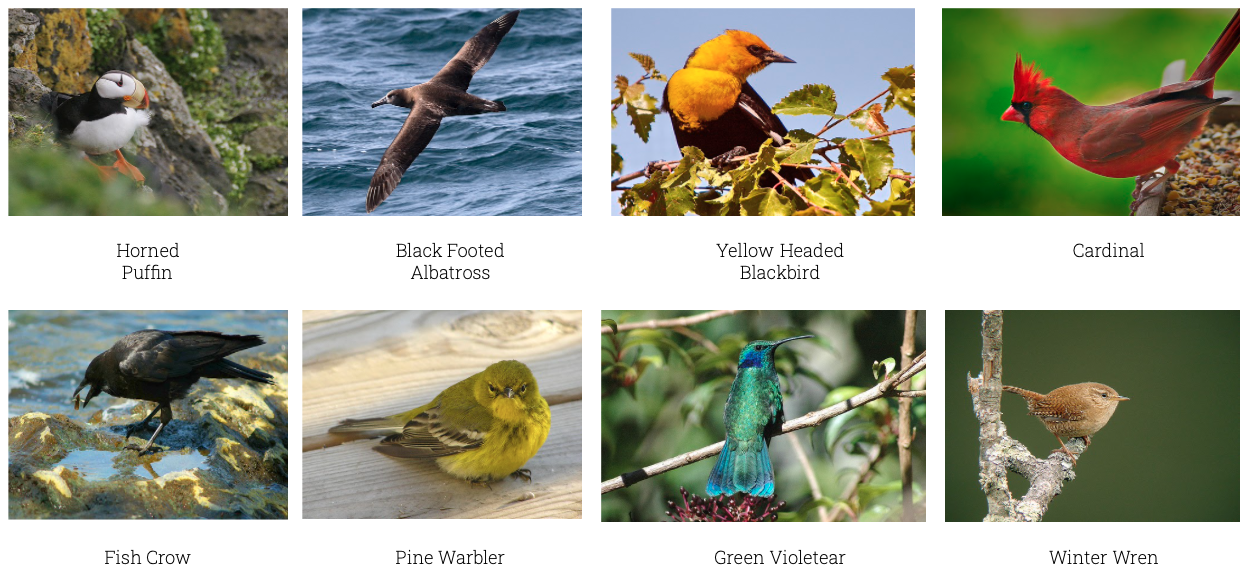
\includegraphics[width=\textwidth]{MS-Thesis-master/figures/cub_new.png}
\caption{A few labelled images from the Caltech-UCSD Birds (CUB) data set.}
\label{image:cub}
\end{figure}

\subchapter{Scene Understanding with Attributes Database (SUN)}
The Scene Understanding with Attributes database (SUN)~\cite{sun} is the first large-scale scene attributes database. A crowd-sourced human study was used to establish a taxonomy of 102 discriminating attributes and the SUN attributes database was built on top of the fine-grained SUN categorical database. The SUN attributes database covers 717 categories and has 14,340 images. SUN is considered a fine-grained data set that is of medium scale in terms of number of images but large scale in terms of number of classes. This data set allows evaluation of the proposed approach in a fine-grained domain with a large number of classes. Few examples of scene classes in SUN are \textit{street}, \textit{indoor brewery}, \textit{valley}, \textit{classroom}, and \textit{supermarket}. The SUN data set also provides a two-level hierarchy for each of the 717 categories. The first level classifies scenes into broad categories such as \textit{indoor}, \textit{outdoor-natural}, and \textit{outdoor-man-made}. The second level further classifies each of the first-level scenes into finer categories such as \textit{workplace}, \textit{shopping}, \textit{forest}, \textit{sports}, \textit{cultural} etc. Figure \ref{image:sun} shows a few images from the SUN data set. The SUN data set is publicly available and further information about the data set can be found here 
\footnote{http://cs.brown.edu/~gmpatter/sunattributes.html}.

\bigskip
\bigskip

\begin{figure}[ht]
\centering
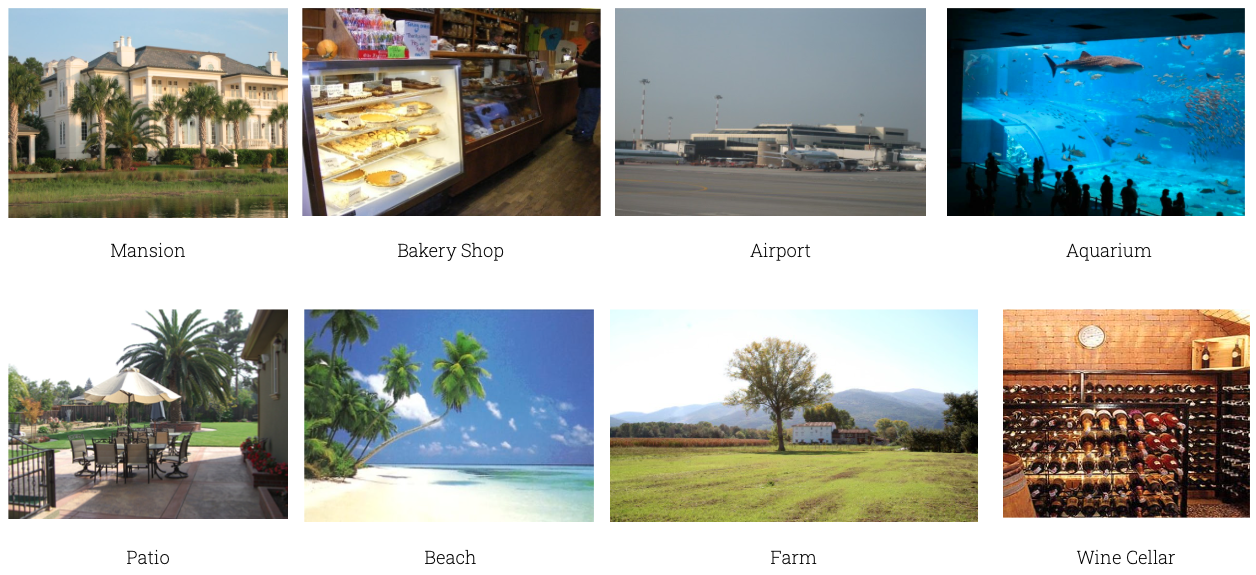
\includegraphics[width=\textwidth]{MS-Thesis-master/figures/sun_new.png}
\caption{A few labelled images from the Scene Understanding with Attributes (SUN) data set.}
\label{image:sun}
\end{figure}


\bigskip
\bigskip

\begin{table}[h]
\centering
\caption{Summary Statistics for all three Data Sets}
\begin{tabular}{@{}lllll@{}}
\toprule
\textbf{Data set} & \textbf{Detail} & \textbf{Classes} & \textbf{Images} & \textbf{Attributes} \\ \midrule
AWA2             & coarse          & 50               & 37,322          & 85\\
CUB              & fine            & 200              & 11,788          & 312\\
SUN              & fine            & 717              & 14,340          & 102\\ \bottomrule
\end{tabular}
\label{table:data_stats}
\end{table}
% Chapter 4: Methodology
\chapter{}{{Methodology}}{Methodology}

Broadly, the proposed framework comprises of the following components:
\begin{enumerate}
    \item Deep feature extraction
    \item Incorporation of auxiliary information
    \item Clustering of auxiliary Information
    \item Multi-label classification of deep features
    \item Predictions of categories/classes
\end{enumerate}

Generally speaking, raw input images carry excess information that is not necessary for the purpose of discrimination and/or fine-grained analysis. Feature extraction enables us to collect important relevant features from an image while discarding the unnecessary information. The deep feature extraction component uses deep neural networks to extract essential information from each image. The first section in this chapter details the feature extraction procedure. Auxiliary information is used by ZSL techniques to learn the relationships between the seen and unseen classes. The second section in this chapter describes the various types of auxiliary information used within the proposed framework. In order to identify representative classes that enable us to predict the large number of unseen classes, we cluster the auxiliary information to find representative cluster centers. The third section in this chapter details the various clustering techniques used. A multi-label classifier is then trained which can discriminate between the representative classes identified in the clustering phase. The fourth section in this chapter describes the classifiers used and their parameters. For a test sample, once the appropriate representative cluster is identified, predictions about unseen classes are made by using a hypothesis generation procedure based on distance measures in the auxiliary space. The fifth section in this chapter describes the distance metrics used to generate the hypotheses from the auxiliary space. Figure \ref{image:overview} depicts a high-level schematic of all the components in the proposed framework.

\begin{sidewaysfigure}
%\begin{figure}[h]

\centering
%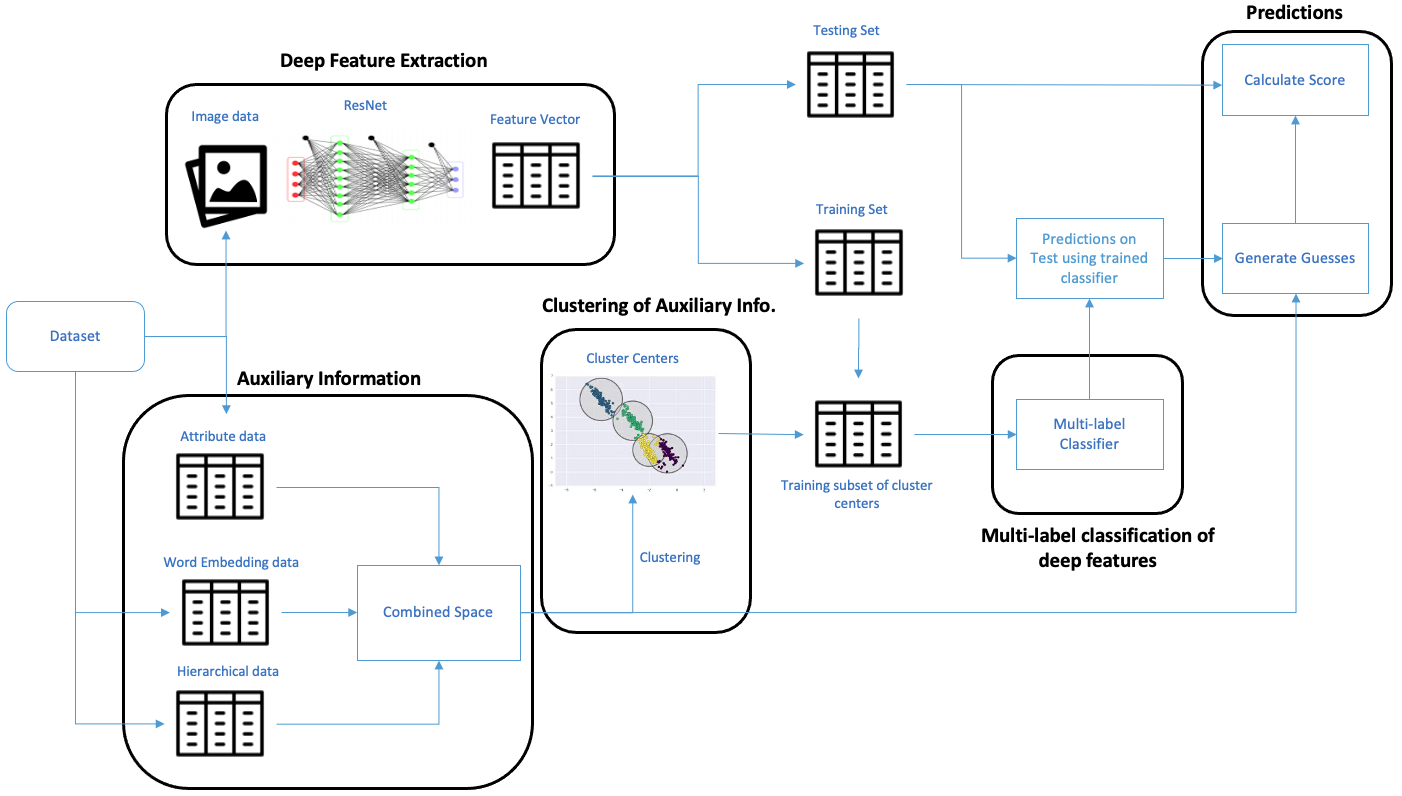
\includegraphics{MS-Thesis-master/figures/overview_new.png}
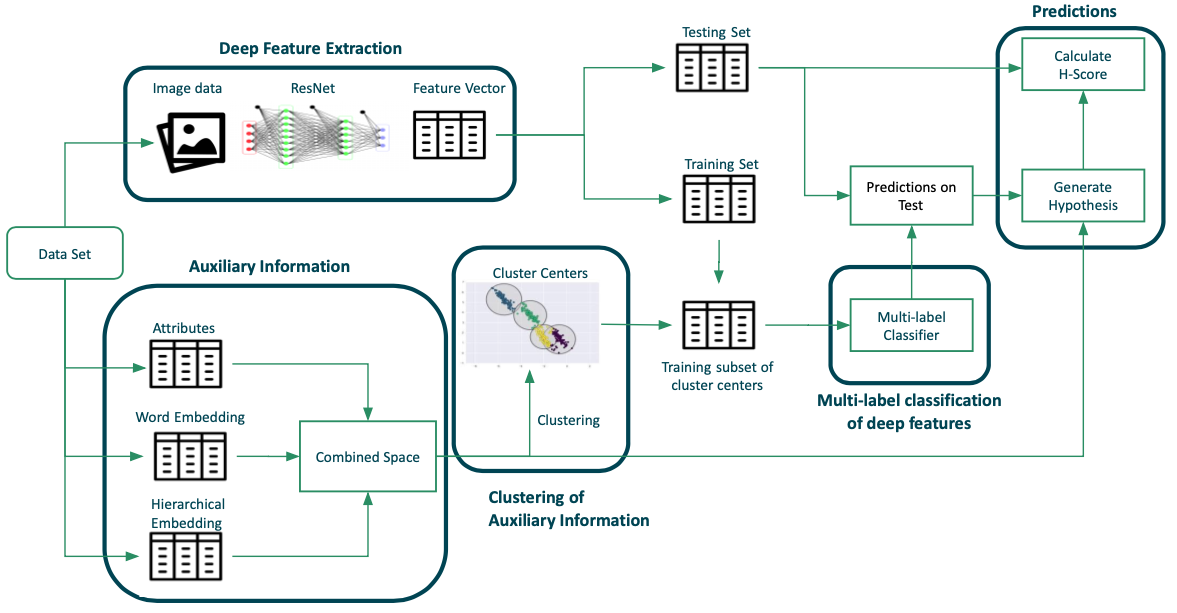
\includegraphics[width=\textwidth]{MS-Thesis-master/figures/overview_latest.png}
%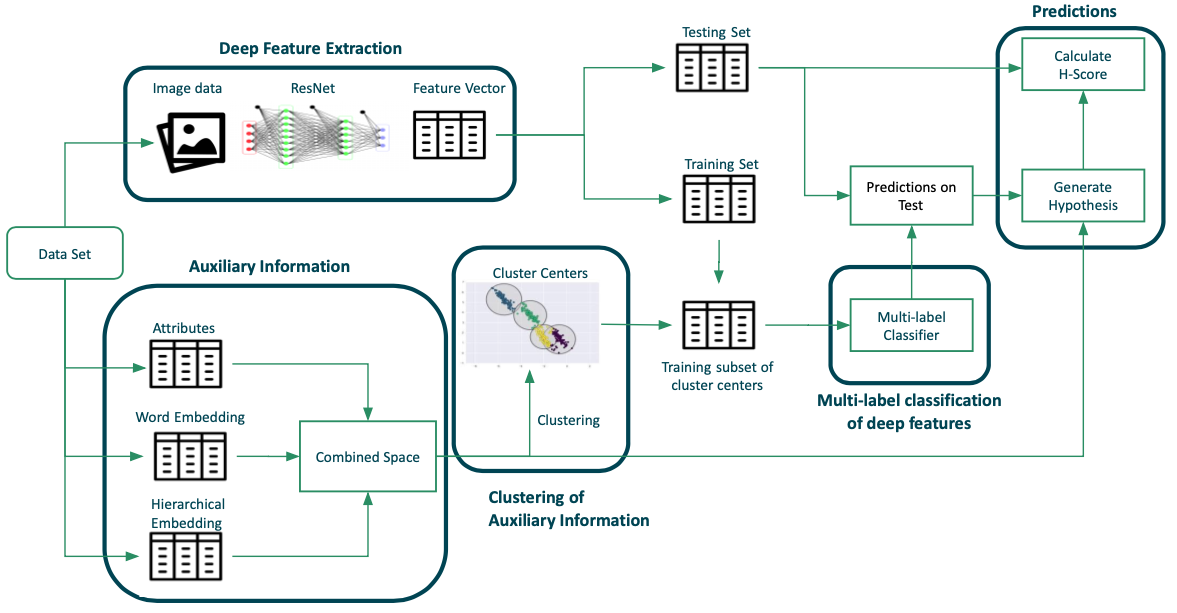
\includegraphics[scale=0.5]{MS-Thesis-master/figures/overview_latest.png}
\caption{High-level schematic of the proposed framework.}
\label{image:overview}
%\end{figure}
\end{sidewaysfigure}

\bigskip
\bigskip

\subchapter{Deep Feature Extraction}

Deep neural networks (DNNs) have proven to perform well for feature extraction from images. We use a ResNet DNN~\cite{resnet} with a depth of 101 layers which is pre-trained on the ImageNet  data set~\cite{imagenet}. This reduces training time significantly and yields useful features since ImageNet consists of over 1 million images spanning 1000 categories. We extract features from the last ResNet layer which translates to 2048 features for each image. ResNet features for all three data sets are also publicly \href{https://www.mpi-inf.mpg.de/departments/computer-vision-and-machine-learning/research/zero-shot-learning/zero-shot-learning-the-good-the-bad-and-the-ugly/}{available}~\cite{gbu}. Figure~\ref{image:resnet_features} shows the architecture and feature extraction map for an image using ResNet-101.

\par
\medskip

Extracted visual features are split into training and testing sets using a stratified 80:20 split. These splits are saved separately for further use in model training and in the prediction phases. Stratified sampling is used so that instances of seen and unseen classes are present in the test set, thus making this a generalized zero-shot learning setting. A seed is used during the splitting phase so that the results can be reproduced. Table \ref{table:train_test_splits} shows a summary of training and testing splits for each data set.

\medskip
\par

\begin{figure}[h!]
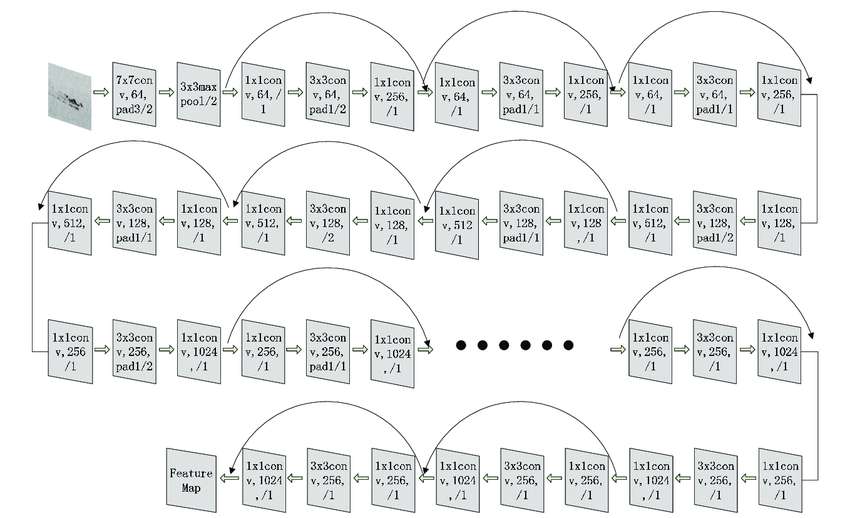
\includegraphics[width=\textwidth]{MS-Thesis-master/figures/ResNet-101-feature-extraction.png}
\caption{ResNet-101 feature extraction map~\cite{resnet-101features}. Each image passes through the network and a feature vector is extracted from the last layer.}
\label{image:resnet_features}
\end{figure}

\par
\medskip

\begin{table}[h!]
\caption{Training and testing splits for each data set}
\centering
\begin{tabular}{@{}lllll@{}}
\toprule
\textbf{Data Set} & \textbf{Classes} & \textbf{Total Images} & \textbf{Training Set Images} & \textbf{Testing Set Images} \\ \midrule
AWA2             & 50               & 37,322          & 29,857                       & 7,465                       \\
CUB              & 200              & 11,788          & 9,430                        & 2,358                       \\
SUN              & 717              & 14,340          & 11,472                       & 2,868                       \\ \bottomrule
\end{tabular}
\label{table:train_test_splits}
\end{table}

\subchapter{Auxiliary Information}

Since instances of unseen classes are unavailable during the training process, auxiliary information is needed to establish semantic relationships between seen and unseen classes, which in turn helps address the ZSL problem. In this framework, we use three sources of auxiliary information for each of the three data sets.

\par
\medskip

\textbf{Attributes.} Humans can naturally perform zero-shot learning with the help of semantic background information. For instance, knowing that "a zebra looks like a horse with stripes" allows us to recognize a zebra without having seen one before, as long as we know what a horse looks like and what the pattern "stripe" looks like \cite{stripes}. All three data sets that are used in this experiment have labelled attribute information for each of their classes. The AWA2 data set~ \cite{awa} includes attributes such as \textit{black}, \textit{small}, \textit{walks}, \textit{smart} etc. with 85 such attributes for each class. The CUB data set ~\cite{cub} includes attributes such as \textit{primary color}, \textit{wing color}, \textit{wing shape}, \textit{size} etc. with 312 such attributes for each class. The SUN data set~\cite{sun} includes attributes such as \textit{man-made}, \textit{natural light}, \textit{medical activity}, \textit{diving} etc. with 102 such attributes for each class.

\par
\medskip

\textbf{Text Embeddings.} A popular idea in modern machine learning is to represent words by vectors that capture hidden information about a language. The learned vector representations for words (i.e., word/text embeddings) from a large general text corpus can help to construct semantic relationships between the seen and unseen class labels. There are three  widely used word embeddings in the research literature: Word2Vec~\cite{w2v}, GloVe~\cite{glove}, and FastText~\cite{fasttext}. FastText has been shown to perform better than the others since it treats each word as composed of character $n$-grams. In FastText the vector for each word is composed as the sum of its character $n$-grams whereas, in Word2Vec and GloVe each word in the corpus is treated as an atomic entity and a unique vector is generated for each word. As a result, FastText can also generate vectors for a combination of words. For instance, "polar bear" has a unique FastText vector representation. FastText has been trained on a very large Wikipedia corpus and is publicly available. In this work, we extract FastText word representations for each class label resulting in a 300-dimensional vector for each class label. 

\par
\medskip

\textbf{Hierarchy Embeddings.} Creating a hierarchy of categories present in a data set allows us to derive taxonomy-based relationships between the classes and improve ZSL performance. For the AWA2 and CUB data sets, Lee et al.~\cite{hnd} propose a two-stage approach for generating hierarchy embeddings where they first derive a top-down hierarchy using WordNet~\cite{wordnet} and then create a flattened hierarchy by representing the probabilities of all the leaf nodes as a single probability vector. Figure~\ref{image:hle} illustrates how hierarchy embeddings are generated for each leaf class in the classification tree. In the case of the AWA2 data set, this results in a 61-dimensional vector and in the case of the CUB data set a 193-dimensional vector. The SUN data set provides its own two-level hierarchy information for each of its 717 categories resulting in a 19-dimensional vector.

\par
\medskip

\begin{figure}[h!]
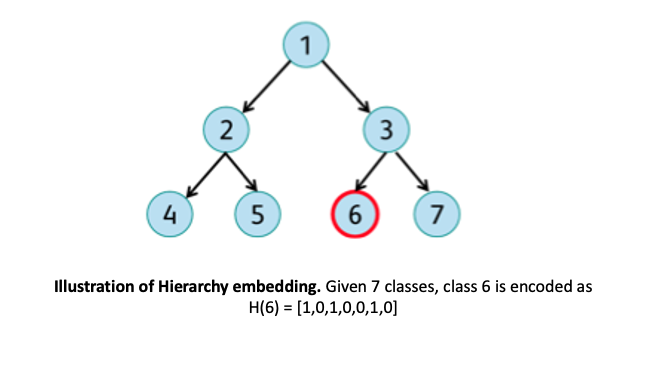
\includegraphics[width=\textwidth]{MS-Thesis-master/figures/hle.png}
\caption{An illustration of hierarchy embedding~\cite{ale}.}
\label{image:hle}
\end{figure}

\textbf{Combined Semantic Space.} The vector spaces of attributes, text embeddings, and hierarchy embeddings are combined into a unified space with reduced dimensions, while retaining the most important information. The dimensionality reduction of the semantic space reduces the computational complexity of the clustering phase and creates robust clusters. We use Principal Component Analysis (PCA) for dimensionality reduction since it retains the variance in the input data while reducing the data dimensionality resulting in a compact combined semantic space. PCA achieves dimensionality reduction by re-projecting the original data along the principal component axes where the principal components are determined via eigenvalue decomposition of the data covariance matrix. The combined, reduced-dimensional semantic space for each data set is computed and retained for use in the clustering and prediction phases. Figures~\ref{image:tsne_awa2}, \ref{image:tsne_cub}, and \ref{image:tsne_sun} show the t-distributed stochastic neighbour embedding (t-SNE) plots~\cite{t-sne} of the combined semantic space for the AWA2, CUB, and SUN data sets respectively. The t-SNE~\cite{t-sne} is a non-linear dimensionality reduction technique that embeds high-dimensional data into a low-dimensional space to aid in data visualization. Specifically, it models each high-dimensional vector as a two- or three-dimensional vector such that similar objects are closer and dissimilar objects are farther apart in the resulting two- or three-dimensional space. In the t-SNE plots for the CUB and SUN data sets, in Figures~\ref{image:tsne_cub} and \ref{image:tsne_sun} respectively, 50 random classes are depicted in the interest of readability. In the t-SNE plots, we observe that classes in the CUB and SUN data set group closer to each other compared to those in the AWA2 data set. This is because AWA2 is a coarse-grained data set whereas CUB and SUN are fine-grained data sets.

\par
\medskip

%\begin{sidewaysfigure}
\begin{figure}[h!]
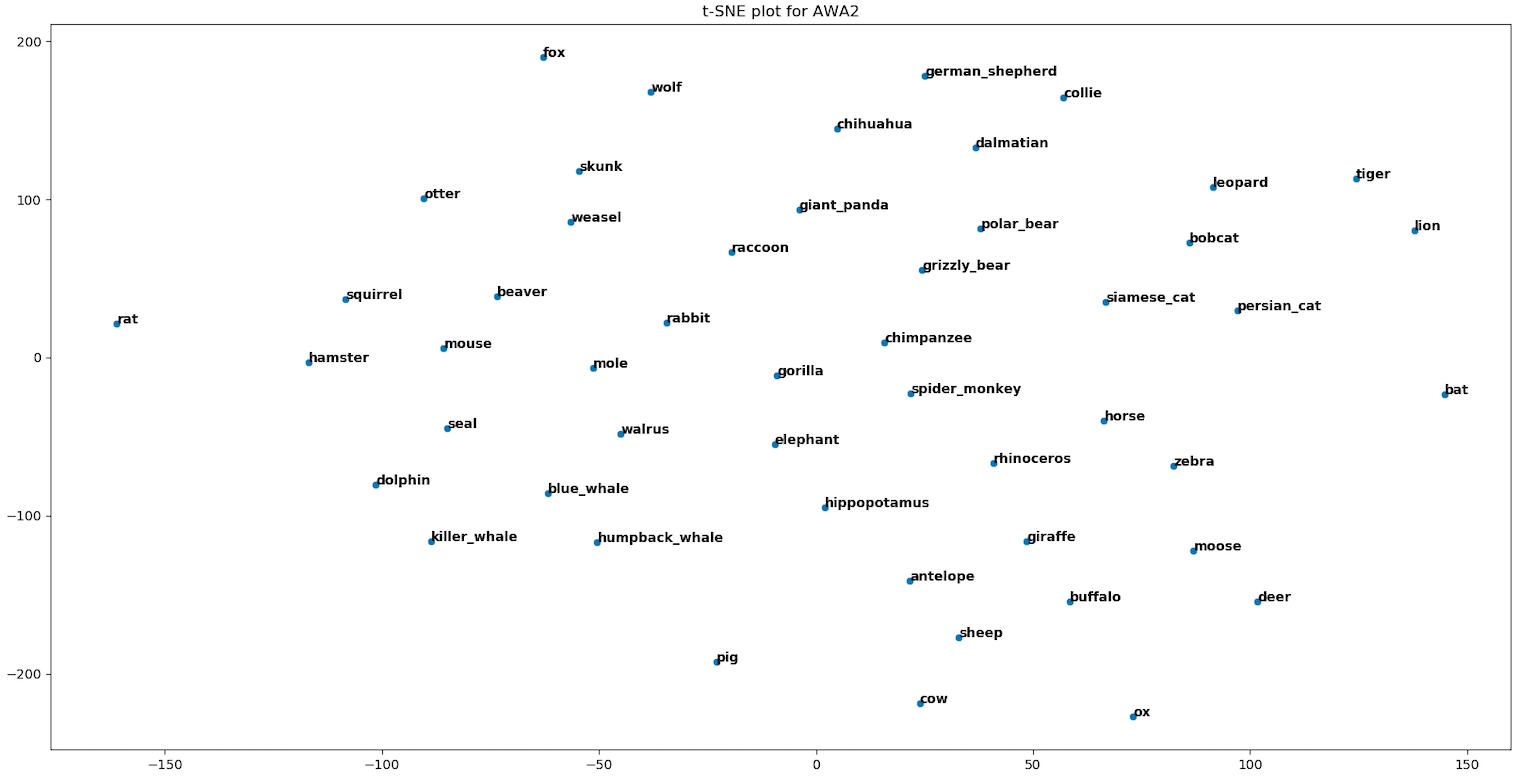
\includegraphics[width=\textwidth]{MS-Thesis-master/figures/tsne_awa2.png}
\caption{t-SNE plot of the combined semantic space in the AWA2 data set with all classes.}
\label{image:tsne_awa2}
\end{figure}

\par
\medskip

%\begin{sidewaysfigure}
\begin{figure}[h!]
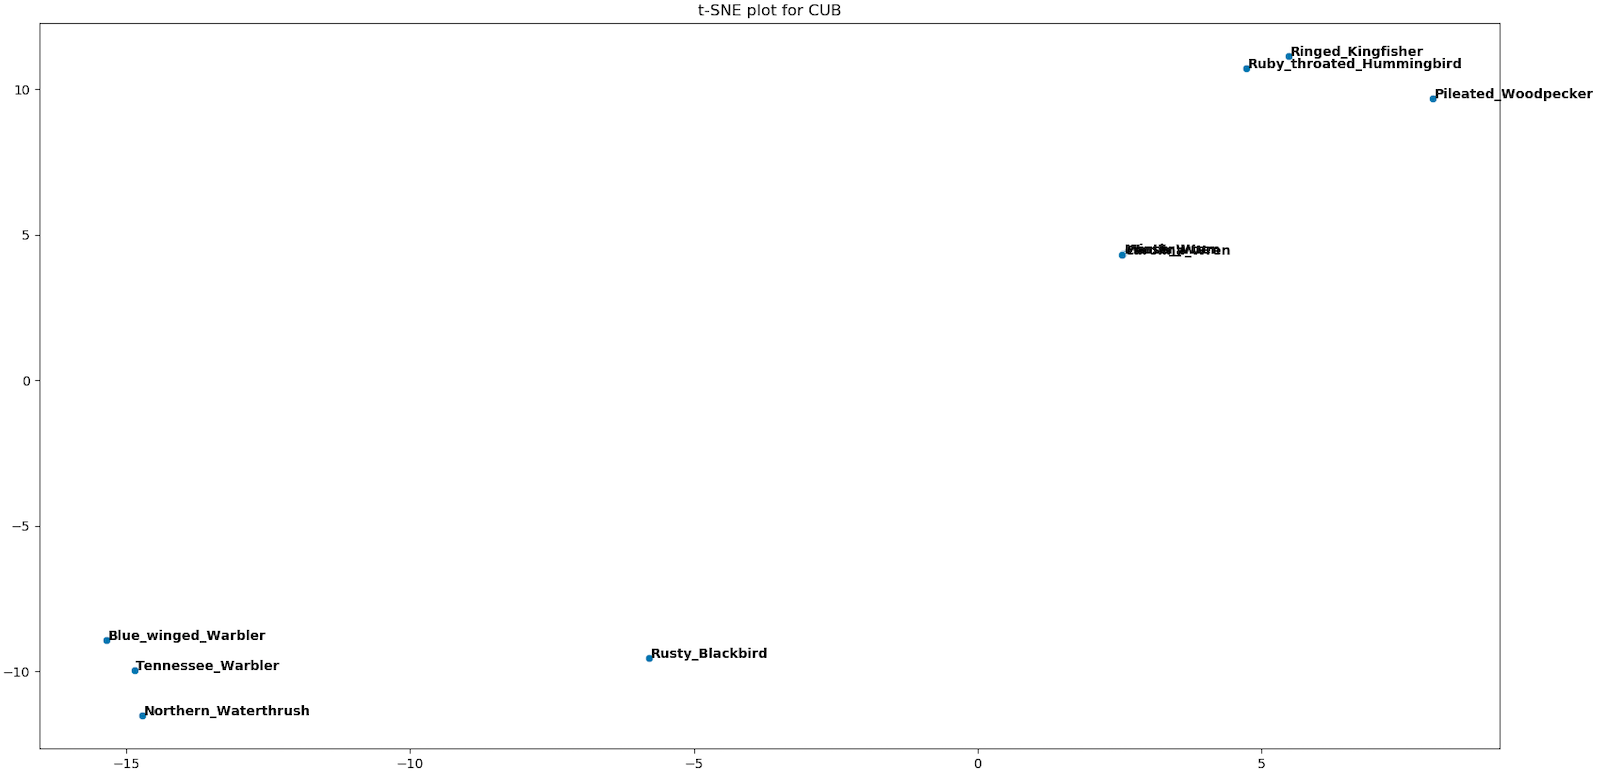
\includegraphics[width=\textwidth]{MS-Thesis-master/figures/tsne_cub_new.png}
\caption{t-SNE plot of the combined semantic space in the CUB data set with 10 classes.}
\label{image:tsne_cub}
\end{figure}

\par
\medskip

\begin{figure}[h!]
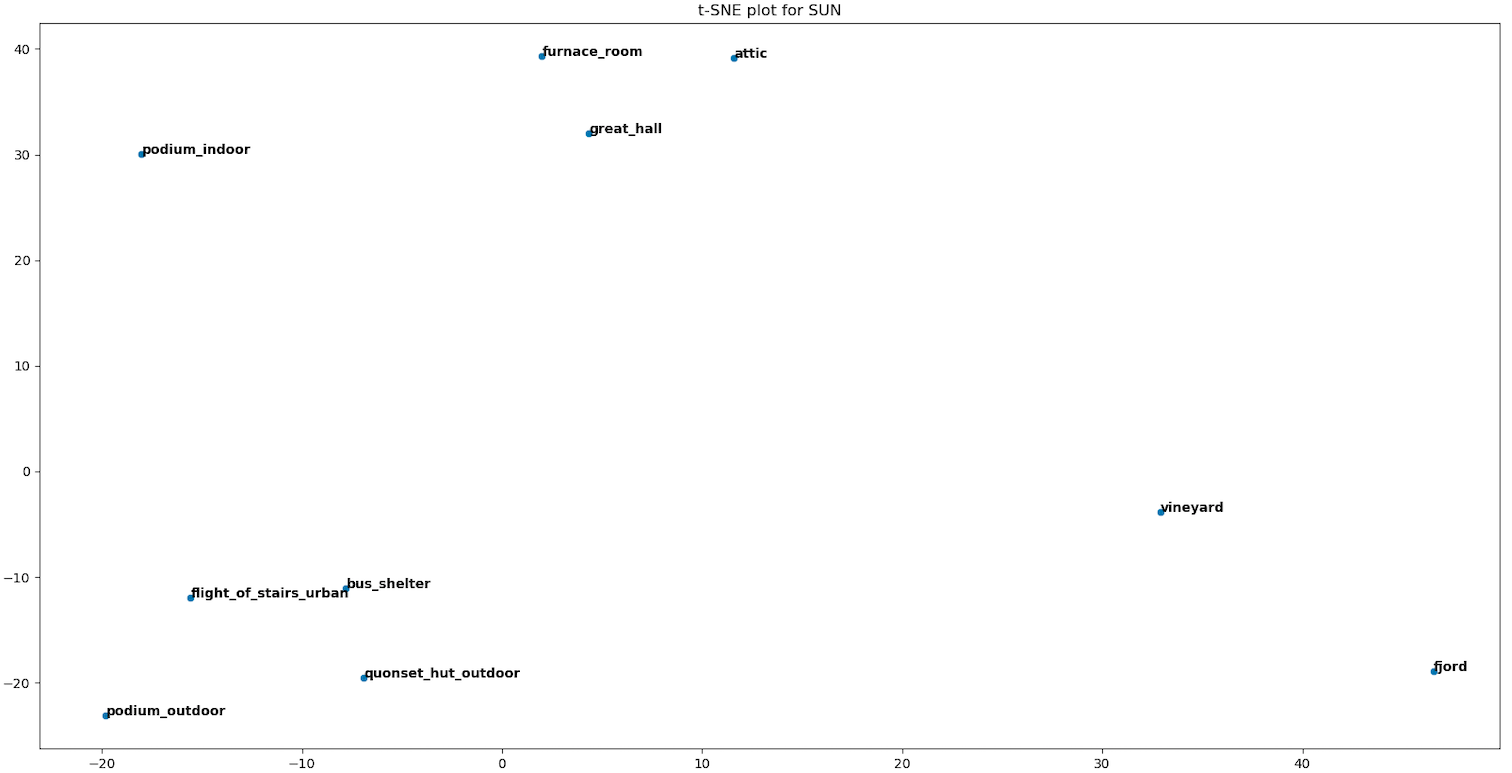
\includegraphics[width=\textwidth]{MS-Thesis-master/figures/tsne_sun_new.png}
\caption{t-SNE plot of the combined semantic space in the SUN data set with 10 classes.}
\label{image:tsne_sun}
\end{figure}

\par
\medskip

\subchapter{Clustering of Auxiliary Information}

The goal of the clustering stage is to identify object categories that are good representatives for a large number of similar object categories. The underlying idea is that these cluster centers would have a strong relationship with its cluster members, thus aiding us to infer cluster members using the cluster centers alone. We use two clustering techniques, i.e., the Gaussian Mixture Model (GMM)~\cite{gmm} and Affinity Propagation (AP)~\cite{affinityprop}, to identify the clusters and representative classes for the clusters. Clustering is performed in the combined reduced-dimensional semantic space for each data set mentioned in the previous section. The clusters centers are noted for further use in the classifier stage.

\par
\medskip

The \textbf{Gaussian Mixture Model (GMM)} can accommodate clusters that have different sizes and correlation structures within them, as opposed to $k$-means clustering. The GMM allows for flexible clustering or soft clustering of the input data. Soft clustering methods assign a score to a data point with respect to each cluster. The value of the score indicates the association strength of the data point to the cluster; in our case the relationship of the data point to the cluster of object categories.  We denote the number of clusters by the variable $k$. GMM-based clustering requires us to specify the number of clusters $k$ before fitting the model. The number of clusters $k$ determines the number of components in the GMM. In our experiments, $k$ starts with a value 5 and ends with a value that equals the total number of classes for a given data set in steps of 5. After identifying all the clusters, the silhouette score~\cite{sil-score} is used to find the optimal value of $k$ for the GMM. 
%%% SMB: ADD THE FOLLOWING CITATION AND REFERENCE FOR silhouette score
%%% P.J. Rousseeuw, Silhouettes: A graphical aid to the interpretation and validation of cluster analysis, Jour. Computational and Applied Mathematics, Vol. 20, 1987, pp. 53-65.

\par
\medskip

\textbf{Affinity Propagation (AP)} is a clustering algorithm based on concept of "message passing" between data points. Unlike the GMM, AP does not require us to specify in advance the number of clusters $k$ to be determined, the algorithm itself provides the optimal number of clusters, i.e., the value of $k$. AP discovers "exemplars" that are members of the input set that are representative of the clusters.

\par
\medskip

The optimal number of clusters for each data set using both clustering techniques is shown in Table \ref{table:k_cl}. It should be noted that since GMM-based clustering was performed using a step size of 5 for $k$, these results may not be the true optimal values for $k$. In this work, we focus primarily on the GMM-based clustering technique since we would like to study how changing number of seen classes i.e. the value of $k$, impacts the classification accuracy.

\par
\medskip

\begin{table}[h!]
\begin{center}
\caption{Optimal number of clusters ($k$ value) for each clustering technique.}
\begin{tabular}{llll}
\hline
\textbf{Data Set} & \textbf{$k$-GMM} & \textbf{$k$-AP} & \textbf{Total Classes} \\ \hline
AWA2 & 15 & 15 & 50\\
CUB & 25 & 24 & 200\\
SUN & 35 & 31 & 717\\ \hline
\end{tabular}
\label{table:k_cl}
\end{center}
\end{table}

\par
\medskip

\subchapter{Multi-label Classification of Deep Features}

After determining the clusters and the representative object for each cluster for different values of $k$, the next step is to train visual classifiers for each cluster center or representative object. A trained visual classifier is used to classify each new test image into one of the representative objects corresponding to the clusters.

\par
\medskip

For each value of $k$, the training set is filtered for the class labels associated with the cluster centers. For example, in the AWA2 data set, for $k = 5$, we have class labels \textit{chimpanzee}, \textit{hamster}, \textit{humpback whale}, \textit{bobcat}, and \textit{ox} as the cluster centers. The image features associated with the class labels of cluster centers alone are considered as the training set and a multi-class visual classifier is trained using this training set. Thus, for each value of $k$, a multi-class classifier is trained, with the training data increasing with increasing number of clusters $k$. Algorithm \ref{algo:cluster_train} shows the steps involved in clustering and training process.

\par
\medskip

\textbf{Visual Classifier.} There are a number of machine learning techniques one can employ to design a multi-class visual classifier such as logistic regression, decision tree, support vector machine (SVM), and neural network. In this work we use a Random Forest (RF) classifier. The RF classifier builds an ensemble of decision trees using a bagging ensemble technique. Simply put, RF builds multiple decision trees and then merges them together to get a more accurate and stable prediction. We use an RF classifier since it is highly scalable for a large number of classes and yields good results. Since we have to train multiple classifiers for varying values of $k$, when using GMM-based clustering, it is difficult to train a neural network or an SVM because of the time complexity and parameter tuning involved. The parameters used in the training of the RF are mentioned in Appendix A.
 
\par
\medskip

\begin{algorithm}[ht]
\SetAlgoLined
\KwData{Combined semantic space, Training set of image features}
\KwResult{Cluster centers and a Trained visual classifier}
 initialization\;
 N $\leftarrow$ Total number of classes in data set\;
 \If{clusteringTechnique = GMM}{
   \For{k in 1 to N with increments of 5}{
  Perform GMM clustering on combined semantic space using k = \textit{k}\;
  Seen classes $\leftarrow$ List of cluster centers\;
  Training subset $\leftarrow$ Subset entire training set for Seen classes alone\;
  Train visual classifier using Training subset\;
  Save classifier
   }
   }
   \If{clusteringTechnique = AF}{
   Perform AF clustering on combined semantic space\;
   Seen classes $\leftarrow$ List of cluster centers\;
   Training subset $\leftarrow$ Subset entire training set for Seen classes alone\;
   Train visual classifier using Training subset\;
   Save classifier
 }
 \caption{Clustering of semantic space and training of visual classifiers. Here, clusteringTechnique denotes the type of clustering technique used. The visual classifier used is a random forest.}
 \label{algo:cluster_train}
\end{algorithm}

\par
\medskip
 
\subchapter{Generation of Predictions or Alternative Hypotheses}
Once visual classifiers are trained, each test instance is classified into one of the representative clusters for a given value of $k$. Alternative hypotheses or predictions are then generated using a similarity measure within the combined semantic space.

\par
\medskip
 
\textbf{Similarity measures.} In machine learning, a similarity measure is an inverse distance metric with dimensionality determined the class feature space. If the distance between two data points is small then there is a high degree of similarity between the classes and vice versa. There are a number of similarity measures using in machine learning such as ones based on Euclidean distance, Manhattan distance, Jaccard distance, and cosine similarity. In this work, we use the cosine similarity measure which computes the cosine of the angle between two vectors as shown in Equation~(\ref{eq:cosine_sim}). Cosine similarity is advantageous because even if the two classes are far apart based on a standard distance metric, it may be possible for their corresponding vectors to be oriented closer together in terms of their angular separation. The smaller the angular separation between the two vectors, the higher the cosine similarity measure.

\par
\medskip
 
\begin{equation}
\label{eq:cosine_sim}
\cos ({\bf a},{\bf b})= {{\bf a} {\bf b} \over \|{\bf a}\| \|{\bf b}\|} = \frac{ \sum_{i=1}^{n}{{\bf a}_i{\bf b}_i} }{ \sqrt{\sum_{i=1}^{n}{({\bf a}_i)^2}} \sqrt{\sum_{i=1}^{n}{({\bf b}_i)^2}} }
\end{equation}

\par
\medskip
 
\textbf{Testing.} Algorithm \ref{algo:test} shows the steps involved in the prediction phase. The test set is split into two subsets. The first subset denotes the seen classes, comprising of data pertaining to class labels that are present in the training set. The second subset denotes the unseen classes, comprising of data pertaining to class labels that are absent from the training set. For each of these subsets, we determine top prediction using the trained visual classifier and then find the closest class label in the combined semantic space using the cosine similarity measure. Classification accuracy is computed for each subset separately followed by the computation of the \textit{harmonic score} (H-score) using Equation~(\ref{eq:hscore}).

\par
\medskip
 
\begin{equation} 
\label{eq:hscore}
\ H-score= \frac{2 *(Seen Class Accuracy)*(Unseen Class Accuracy)}{(Seen Class Accuracy)+(Unseen Class Accuracy)}\
\end{equation}

\par
\medskip
 
We choose the harmonic mean as the performance metric instead of the arithmetic mean because in the case of the latter, if the seen class accuracy is much higher than the unseen class accuracy, the overall arithmetic mean is significantly skewed towards the seen class accuracy~\cite{gbu}. However, since our aim is to attain high classification accuracy on both the seen and unseen classes, the harmonic mean is a better quantifier of overall classification accuracy.

\par
\medskip
 
\begin{algorithm}[ht]
\SetAlgoLined
\KwData{Combined semantic space, Trained Classifiers, Trained Clusters, Testing set of image features}
\KwResult{Overall H-Score on the test set}
 initialization\;
 N $\leftarrow$ Total number of classes in data set\;
 C $\leftarrow$ List of all class labels in data set\;
 \If{clusteringTechnique = GMM}{
   \For{k in 1 to N with increments of 5}{
  Cluster centers $\leftarrow$ List of cluster centers from clusters trained using k = \textit{k}\;
  Seen classes $\leftarrow$ Subset test set for Cluster centers alone\;
  Unseen classes $\leftarrow$ Subset test set for  [C - Cluster centers]\;
  Use classifier trained for k=\textit{k} to predict on seen and unseen classes\;
  Use cosine similarity to find closest neighbour in Combined semantic space\;
  Calculate accuracy\;
  Calculate H-Score\;
   }
   }
   \If{clusteringTechnique = AF}{
  Cluster centers $\leftarrow$ List of cluster centers from clusters trained using k = \textit{k}\;
  Seen classes $\leftarrow$ Subset test set for Cluster centers alone\;
  Unseen classes $\leftarrow$ Subset test set for  [C - Cluster centers]\;
  Use classifier trained for k=\textit{k} to predict on seen and unseen classes\;
  Use cosine similarity to find closest neighbour in Combined semantic space\;
  Calculate accuracy\;
  Calculate H-Score\;
 }
 \caption{Prediction phase algorithm. Here, clusteringTechnique denotes the type of clustering technique used.}
 \label{algo:test}
\end{algorithm}

\newpage
% Chapter 3: Comparison
\chapter{}{{Experimental Results and Discussion}}{Experimental Results and Discussion}

As stated in Chapters 1 and 2, the experimental setup in the proposed approach differs from the standard ZSL setup. The proposed approach aims to minimize the number of seen classes within a data set while delivering reasonable performance on the unseen classes. This makes it hard to compare our results with those of other ZSL frameworks mentioned in the research literature. In order to achieve a fair comparison of the proposed framework with other ZSL approaches, we modify a well known ZSL framework to work with our experiment setup. 

\par
\medskip
 
\textbf{Attribute Label Embedding (ALE)} \cite{ale} uses a bi-linear compatibility function to associate visual and auxiliary information. It embeds each class in the space of attribute vectors. The approach also generalizes to any type of auxiliary information that can be encoded in matrix form such as word embeddings. A comparison study performed in \cite{gbu} shows that ALE outperforms other ZSL frameworks in the generalized ZSL setting. Recent generative methods described in the literature could potentially perform better than ALE but such a comparison study using same data sets, experimental conditions, and evaluation metrics has not been performed yet. Hence, we chose to compare the proposed approach with the ALE framework. A working implementation of the ALE framework was obtained from a recent GitHub repository \footnote{https://github.com/cetinsamet/attribute-label-embedding}
and modified to work within our experimental setting. Once the clusters centers are determined for each value of $k$, the ALE procedure is performed on the appropriate training and testing sets. Table~\ref{table:gmm_com} and Table~\ref{table:af_com} show a summary of the comparison between the proposed approach and ALE using both clustering techniques, i.e., GMM-based clustering and AP-based clustering. Table~\ref{table:full_results} in Appendix B provides comprehensive results on all three data sets when using GMM-based clustering.

\par
\medskip
\noindent 
\textbf{Results on the AWA2 data set.} The AWA2 data set has 50 classes and the training set consists of 560 images per class on average with the category \textit{horse} having the highest number of images (1316), and  the category \textit{mole} having the least number of images (80). 

We study performance of the proposed approach for $k = 25$ which renders half the classes as seen and half the classes as unseen for the model. The seen classes exhibit an average classification accuracy of 85\% whereas the unseen classes exhibit an average classification accuracy of 27\% on the test set. 

Among the seen classes, we find there are three cases:

\begin{enumerate}[label=Seen Case: \arabic*]
    \item Seen classes exhibiting $\geq 90\%$ classification accuracy on the test set. In the AWA2 data set, 16 of 25 seen classes fall in this category and are expected to aid very well in the inference of unseen classes related to these seen classes. These seen classes have a good number of images to train on and the classifier is able to clearly identify distinguishing features for each class. For example, \textit{humpback whale} is a seen class that exhibits 100\% classification accuracy on the test set. Ideally, we would want all seen classes to fall into this category.
    
    \item Seen classes exhibiting classification accuracy $\geq 60\%$ but $< 90\%$ on the test set. In the AWA2 data set, 7 of 25 seen classes fall in this category and are expected to aid reasonably in the inference of unseen classes. Although these classes have a reasonable number of images to train on, these classes fall into a case where the classes are very close to each other but are still seen classes. For example, \textit{ox}, \textit{moose}, and \textit{cow} fall in this category. It is understandable why the visual classifier would not be able to clearly distinguish between these categories, they are quite similar compared to other categories in this data set.  
    
    \item Seen classes exhibiting classification accuracy $ < 60\%$ on the test set. In the AWA2 data set, 2 of 25 seen classes fall in this category and are expected to negatively impact the unseen class inference process. These 2 classes have only an average of 160 images in the training set, hence the visual classifiers were not be trained enough on these classes to learn the discriminating features.
\end{enumerate}

\par
\medskip

Among the unseen classes also we find three cases:

\begin{enumerate}[label=Unseen Case: \arabic*]
    \item Unseen classes exhibiting $>60\%$  classification accuracy on the test set. In the AWA2 data set, 6 of 25 unseen classes fall in this category. These are cases when a particular unseen class is inferred from a seen class falling in Case 1 of seen classes. For example, \textit{blue whale} is an unseen class that exhibits 100\% accuracy on the test set, and it is inferred from \textit{humpback whale} which falls under Case 1 of the seen classes.
    
    \item Unseen classes exhibiting classification accuracy $\geq  1\%$  but $\leq 60\%$ on the test set. In the AWA2 data set, 6 of 25 unseen classes fall in this category. These are cases where the unseen classes are inferred from the seen classes falling in Case 2 and Case 3 of seen classes. These unseen classes exhibit poor performance since the seen classes they are inferred from are not clearly distinguishable by the visual classifier. For example, \textit{deer} is an unseen class that is inferred from the seen class \textit{moose} which falls in Case 2 of the seen classes.
    
    \item Unseen classes that exhibit $0\%$ accuracy on the test set. In the AWA2 data set, 12 of 25 unseen classes fall in this category. Since our inference process only allows for guessing 1 unseen class per seen class, unseen classes that are farther away from seen classes cannot be inferred and fall in this category. For example, \textit{antelope} is an unseen class that falls in the cluster of \textit{moose}, but only \textit{deer} can be inferred from \textit{moose} since it is the closest neighbor to \textit{moose} based on the cosine similarity measure.
\end{enumerate}

\par
\medskip

The proposed model performs well when a seen class has a sufficient number of images to train on and the unseen class being inferred from it is proximal to the seen class and it performs poorly when the unseen class being inferred is distant from any of the representative classes. Ideally, the proposed model would perform best when there are clusters of size 2 and the representative object for the cluster has clear discriminating features, while the unseen class in the cluster is also closer to the representative class than any other class. Figure~\ref{image:awa2_comparison} shows a comparison of the H-scores obtained on the AWA2 data set by the proposed model and ALE for all values of $k$. As seen from the graph, our model performs significantly better than ALE for all values of $k$ on this data set. The H-score keeps increasing as the value of $k$ increases which is expected since the number of seen classes increase which enables more unseen classes to be inferred more accurately. 

\par
\medskip

In order to determine the optimal numbers of classes required to achieve reasonable performance, we choose a $k$ value for which we achieve a greater than average H-score performance with the proposed model. For $k = 20$, we achieve a H-score of 46\% with the proposed model whereas the average H-score on the AWA2 data set is 45\% across all categories. Thus, on the AWA2 data set, we need to have at least 20 categories as seen classes to reasonably infer the unseen classes with greater than average accuracy with the proposed model.

\par
\medskip

\begin{figure}[h]
\centering
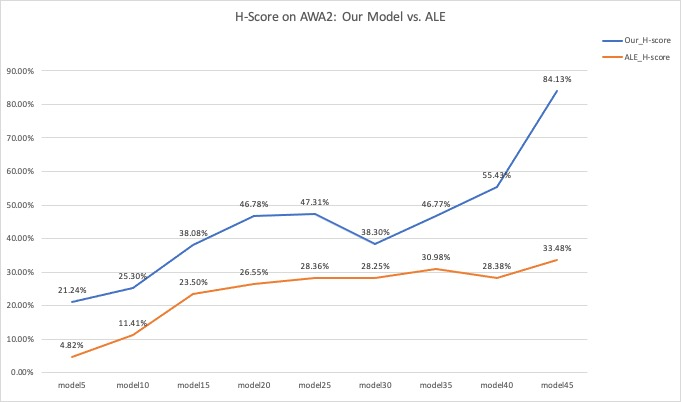
\includegraphics[width=\textwidth]{MS-Thesis-master/figures/awa2_comparison.jpg}
\caption{H-score comparison between the proposed model and ALE on AWA2 data set when using GMM-based clustering.}
\label{image:awa2_comparison}
\end{figure}

\par
\medskip
\noindent
\textbf{Results on the CUB data set.} The CUB data set has 200 classes with 47 images per class on average in the training set. This is a small number of images to train on for each seen class. However, the proposed model still performs well on this data set. 

\par
\medskip

Figure~\ref{image:cub_comparison} shows a comparison of H-scores obtained on the CUB data set using the proposed model and ALE for all values of $k$. As seen from the graph, the proposed model performs better than ALE for values of $k \leq 65$. For $65 < k \leq 115$, the proposed model and ALE exhibit comparable performance and for $k > 115$, the proposed model significantly outperforms ALE on the CUB data set. Thus, across a large range of $k$ values, the proposed model performs better than ALE on the CUB data set. 

\par
\medskip

For $k = 80$, we achieve a H-score of 33.5\% with the proposed model whereas the average H-score on the CUB data set is 33\% across all categories. Thus, on the CUB data set, we need to use at least 80 categories as seen classes to reasonably infer the unseen classes with higher than average accuracy with the proposed model.

\par
\medskip

\begin{figure}[h]
\centering
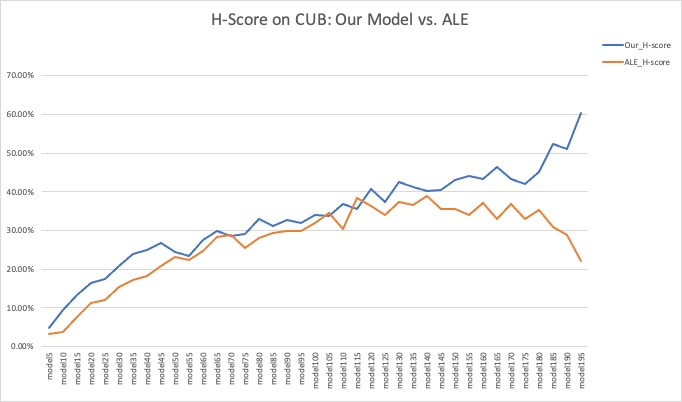
\includegraphics[width=\textwidth]{MS-Thesis-master/figures/cub_comparison.jpg}
\caption{H-score comparison between the proposed model and ALE on CUB data set when using GMM-based clustering.}
\label{image:cub_comparison}
\end{figure}

\par
\medskip
\noindent
\textbf{Results on the SUN data set.} The SUN data set has 717 classes with 16 images per class on average in the training set. This makes it hard for the visual classifier to learn distinguishing features for each class because of the large number of classes and small number of images for each class. Nevertheless, the proposed model exhibits performance that is comparable to ALE on this data set. Figure~\ref{image:sun_comparison} shows a comparison of H-scores obtained on the SUN data set using the proposed model and ALE for all values of $k$. As seen from the graph, ALE performs better than the proposed model for values of $k \leq 560$ and the proposed model performs better than ALE for values of $k$ beyond 560.

\par
\medskip

For $k = 360$, we achieve a H-score of 22\% with the proposed model and the average H-score on the CUB data set is 21.6\% across all categories. Thus, on the SUN data set, we need to use at least 360 categories as seen classes to reasonably infer the unseen classes with greater than average accuracy with the proposed model.

\par
\medskip

\begin{figure}[h]
\centering
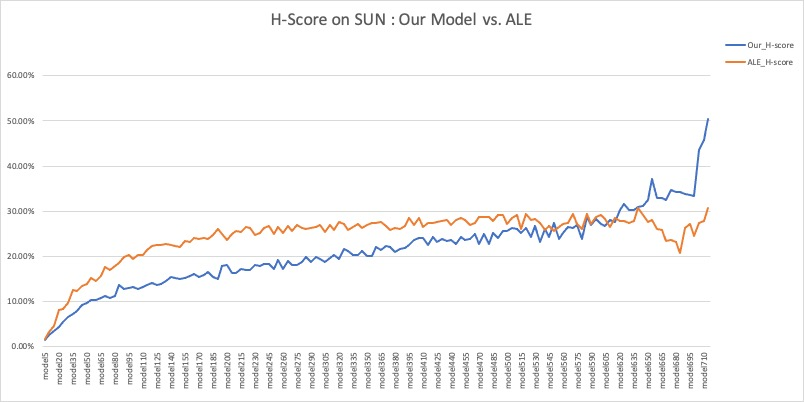
\includegraphics[width=\textwidth]{MS-Thesis-master/figures/sun_comparison.jpg}
\caption{H-score comparison between the proposed model and ALE on SUN data set when using GMM-based clustering.}
\label{image:sun_comparison}
\end{figure}

\par
\medskip

\begin{table}[h]
\caption{Comparison of average classification accuracy across $k$ values between the proposed model and ALE when using GMM-based clustering.}
\centering
\begin{tabular}{@{}lllllll@{}}
\toprule
\textbf{}        & \multicolumn{3}{c}{\textbf{Proposed Model}}                            & \multicolumn{3}{c}{\textbf{ALE}}                                  \\ \midrule
\textbf{Data Set} & \textbf{Avg. Seen} & \textbf{Avg. Unseen} & \textbf{Avg. H-Score} & \textbf{Avg. Seen} & \textbf{Avg. Unseen} & \textbf{Avg. H-Score} \\
AWA2             & 94\%               & 32\%                 & \textbf{45\%}         & 90\%               & 14\%                 & 24\%                  \\
CUB              & 78\%               & 22.86\%              & \textbf{33\%}         & 70\%               & 17.50\%              & 27.19\%               \\
SUN              & 58.20\%            & 15\%                 & 21.60\%               & 41.50\%            & 17.80\%              & \textbf{25\%}         \\ \bottomrule
\end{tabular}
\label{table:gmm_com}
\end{table}

\par
\medskip

\begin{table}[ht]
\caption{Comparison of average classification accuracy between the proposed model and ALE when using AP-based clustering.}
\centering
\begin{tabular}{@{}lllllll@{}}
\toprule
                 & \multicolumn{3}{c}{\textbf{Proposed Model}}             & \multicolumn{3}{c}{\textbf{ALE}}                   \\ \midrule
\textbf{Data Set} & \textbf{Seen} & \textbf{Unseen} & \textbf{H-Score} & \textbf{Seen} & \textbf{Unseen} & \textbf{H-Score} \\
AWA2             & 96.44\%          & 23.43\%         & \textbf{37.7\%}    & 83.40\%       & 10\%            & 17.50\%          \\
CUB              & 91\%          & 9.70\%          & \textbf{17.50\%} & 55\%          & 8.33\%          & 14.40\%          \\
SUN              & 83.10\%       & 4.30\%          & 8.20\%           & 24.40\%       & 8.20\%          & \textbf{12.30\%} \\ \bottomrule
\end{tabular}
\label{table:af_com}
\end{table}

\par
\bigskip
\bigskip
\noindent
\textbf{Hardware Specifications.} All the experiments were performed on an Intel I7 6850K CPU with 128GB RAM. For the AWA2 data set, it takes $\approx$ 20 minutes to train visual classifiers for all values of $k$.  Likewise, for the CUB and SUN data sets, it takes $\approx$ 2.5 hours and $\approx$ 40 hours, respectively, to train visual classifiers for all values of $k$.





\newpage
% Chapter 3: Conclusion
\chapter{}{Conclusions and Future Work}{Conclusions and Future Work}

In this thesis, we propose a framework for generalized zero-shot learning (ZSL) that is simple yet very effective. The proposed framework offers an intuitive approach to aid in the training data collection process for image recognition tasks by identifying representative classes using various clustering techniques. It also  provides a method to infer unseen classes using cosine similarity measure. The proposed framework achieves accuracy figures that are 21\% greater on the AWA2 data set and 6\% greater on the CUB data set when compared to the well known Attribute Label Embedding (ALE) scheme for GZSL. On the SUN data set, the proposed model exhibits performance that is comparable to that of ALE. We also determine the minimum number of categories needed to considered as seen classes to achieve reasonable classification accuracy results on all the three data sets using the proposed model.

\par
\medskip

One of the drawbacks of the proposed framework is the inability to infer unseen classes that are distant from the representative classes in the semantic space. There is significant scope for future improvement of the proposed framework in this aspect. A potential solution could be a scheme to map the distance between each unseen class and representative class in a cluster to the classification probabilities obtained from the visual classifier. In this way, the framework would be able to infer all unseen classes, regardless of the distance, with some non-zero probability.

\par
\medskip

Another important future task is the evaluation of the proposed framework on a very large data set such as ImageNet. ImageNet spans more than 1000 classes and has several images in each class unlike the SUN data set which while having over 700 classes, has very few images per class.

\newpage

% Add 'References' section to Table of Contents
\addcontentsline{chl}{chapter}{~REFERENCES}
% Print References
\clearpage
\printbibliography[title={%
    \begin{center}
        \normalsize
        \MakeUppercase{\textbf{References}}
    \end{center}}]

% Adding Appendix
\newpage

% Add APPENDIX to Table of Contents
\addcontentsline{chl}{chapter}{~APPENDIX}

% Add APPENDIX sub-chapters to Table of Contents
\addcontentsline{chl}{chapter}
{\qquad\protect\numberline{
    A} \hspace{0.5em} Model Parameters
}

% Print APPENDIX Title
\begin{center}
    \textbf{APPENDIX A}

    \MakeUppercase{\textbf{Model Parameters}}
    \vspace*{\baselineskip}
\end{center}

% Contents:
\subsection*{A.1 \hspace{0.5em} Random Forest}

    \begin{itemize}
    \item \textbf{AWA2} \textit{n\_estimators} : 1000, 
        \textit{max\_depth} : 60, 
        \textit{n\_jobs} : -1,
        \textit{min\_samples\_split} : 2,
        \textit{min\_samples\_leaf} : 1,
        \textit{max\_features} : 'auto',
        \textit{bootstrap} : 'False'
     \item \textbf{CUB} \textit{n\_estimators} : 1000, 
        \textit{max\_depth} : 60, 
        \textit{n\_jobs} : -1,
        \textit{min\_samples\_split} : 2,
        \textit{min\_samples\_leaf} : 1,
        \textit{max\_features} : 'auto',
        \textit{bootstrap} : 'False'
     \item \textbf{SUN} \textit{n\_estimators} : 500, 
        \textit{max\_depth} : 60, 
        \textit{n\_jobs} : -1,
        \textit{min\_samples\_split} : 2,
        \textit{min\_samples\_leaf} : 1,
        \textit{max\_features} : 'auto',
        \textit{bootstrap} : 'False'
    \end{itemize}

\subsection*{A.2 \hspace{0.5em} GMM Clustering}

 \begin{itemize}
     \item \textbf{AWA2} \textit{k} : 5 to 45 with steps of 5
     \item \textbf{CUB} \textit{k} : 5 to 195 with steps of 5
     \item \textbf{SUN} \textit{k} : 5 to 715 with steps of 5
 \end{itemize}

\subsection*{A.3 \hspace{0.5em} Principal Component Analysis}

 \begin{itemize}
     \item \textbf{AWA2} \textit{explained\_variance} : 0.70
     \item \textbf{CUB} \textit{explained\_variance} : 0.40
     \item \textbf{SUN} \textit{explained\_variance} : 0.60
 \end{itemize}

\newpage

\newpage

% Add APPENDIX to Table of Contents
\addcontentsline{chl}{chapter}{~APPENDIX}

% Add APPENDIX sub-chapters to Table of Contents
\addcontentsline{chl}{chapter}
{\qquad\protect\numberline{
    B} \hspace{0.5em} Complete Model Results
}

% Print APPENDIX Title
\begin{center}
    \textbf{APPENDIX B}

    \MakeUppercase{\textbf{Complete Model Results}}
    \vspace*{\baselineskip}
\end{center}

% Please add the following required packages to your document preamble:
% \usepackage{booktabs}
% \usepackage{longtable}
% Note: It may be necessary to compile the document several times to get a multi-page table to line up properly
\begin{longtable}{@{}llllllllll@{}}
\caption{Results on all data sets when using GMM-based clustering}
\label{table:full_results} \\
\toprule
 &
  \multicolumn{3}{c}{\textbf{AWA2}} &
  \multicolumn{3}{c}{\textbf{CUB}} &
  \multicolumn{3}{c}{\textbf{SUN}} \\* \midrule
\endfirsthead

\toprule
 &
  \multicolumn{3}{c}{\textbf{AWA2}} &
  \multicolumn{3}{c}{\textbf{CUB}} &
  \multicolumn{3}{c}{\textbf{SUN}} \\* \midrule
\endhead
%
\bottomrule
\endfoot
%
\endlastfoot
%
\textbf{Model} &
  \textbf{Seen} &
  \textbf{Unseen} &
  \textbf{H\_score} &
  \textbf{Seen} &
  \textbf{Unseen} &
  \textbf{H\_score} &
  \textbf{Seen} &
  \textbf{Unseen} &
  \textbf{H\_score} \\
model5   & 96.72\% & 11.93\% & 21.24\% & 100.00\% & 2.52\%  & 4.92\%  & 90.00\%  & 0.67\%  & 1.33\%  \\
model10  & 96.82\% & 14.55\% & 25.30\% & 97.50\%  & 4.96\%  & 9.44\%  & 100.00\% & 1.20\%  & 2.37\%  \\
model15  & 95.97\% & 23.75\% & 38.08\% & 93.82\%  & 7.11\%  & 13.22\% & 93.33\%  & 1.57\%  & 3.09\%  \\
model20  & 94.10\% & 31.13\% & 46.78\% & 92.80\%  & 9.00\%  & 16.41\% & 87.50\%  & 2.33\%  & 4.54\%  \\
model25  & 93.57\% & 31.66\% & 47.31\% & 86.82\%  & 9.65\%  & 17.37\% & 93.00\%  & 2.64\%  & 5.13\%  \\
model30  & 92.82\% & 24.13\% & 38.30\% & 86.16\%  & 11.83\% & 20.80\% & 90.83\%  & 3.64\%  & 7.00\%  \\
model35  & 92.36\% & 31.31\% & 46.77\% & 85.71\%  & 13.93\% & 23.97\% & 87.86\%  & 3.34\%  & 6.44\%  \\
model40  & 92.07\% & 39.65\% & 55.43\% & 84.86\%  & 14.61\% & 24.93\% & 83.75\%  & 3.51\%  & 6.74\%  \\
model45  & 90.76\% & 78.41\% & 84.13\% & 86.33\%  & 15.90\% & 26.85\% & 80.00\%  & 4.20\%  & 7.98\%  \\
model50  &         &         &         & 81.49\%  & 14.41\% & 24.49\% & 81.00\%  & 3.97\%  & 7.57\%  \\
model55  &         &         &         & 80.19\%  & 13.67\% & 23.36\% & 79.55\%  & 4.38\%  & 8.30\%  \\
model60  &         &         &         & 81.95\%  & 16.62\% & 27.64\% & 80.42\%  & 4.34\%  & 8.24\%  \\
model65  &         &         &         & 81.82\%  & 18.26\% & 29.86\% & 78.46\%  & 5.90\%  & 10.97\% \\
model70  &         &         &         & 81.71\%  & 17.36\% & 28.64\% & 79.29\%  & 5.02\%  & 9.44\%  \\
model75  &         &         &         & 78.71\%  & 17.76\% & 28.98\% & 77.00\%  & 5.72\%  & 10.65\% \\
model80  &         &         &         & 81.66\%  & 20.72\% & 33.05\% & 76.25\%  & 5.30\%  & 9.91\%  \\
model85  &         &         &         & 80.08\%  & 19.28\% & 31.08\% & 73.24\%  & 6.17\%  & 11.38\% \\
model90  &         &         &         & 78.79\%  & 20.66\% & 32.74\% & 73.33\%  & 5.58\%  & 10.37\% \\
model95  &         &         &         & 79.80\%  & 20.02\% & 32.01\% & 73.68\%  & 6.15\%  & 11.35\% \\
model100 &         &         &         & 77.65\%  & 21.84\% & 34.09\% & 71.50\%  & 6.00\%  & 11.07\% \\
model105 &         &         &         & 75.20\%  & 21.79\% & 33.79\% & 69.52\%  & 6.25\%  & 11.47\% \\
model110 &         &         &         & 76.23\%  & 24.29\% & 36.84\% & 65.45\%  & 6.05\%  & 11.08\% \\
model115 &         &         &         & 76.27\%  & 23.08\% & 35.44\% & 69.13\%  & 5.86\%  & 10.80\% \\
model120 &         &         &         & 75.09\%  & 28.03\% & 40.82\% & 68.33\%  & 7.41\%  & 13.37\% \\
model125 &         &         &         & 74.76\%  & 25.00\% & 37.47\% & 67.80\%  & 6.88\%  & 12.49\% \\
model130 &         &         &         & 75.36\%  & 29.59\% & 42.49\% & 65.77\%  & 6.94\%  & 12.56\% \\
model135 &         &         &         & 74.64\%  & 28.46\% & 41.21\% & 70.56\%  & 7.17\%  & 13.02\% \\
model140 &         &         &         & 73.50\%  & 27.63\% & 40.16\% & 68.57\%  & 6.89\%  & 12.52\% \\
model145 &         &         &         & 72.26\%  & 28.02\% & 40.38\% & 65.17\%  & 6.64\%  & 12.05\% \\
model150 &         &         &         & 71.66\%  & 30.68\% & 42.97\% & 62.33\%  & 7.10\%  & 12.75\% \\
model155 &         &         &         & 70.08\%  & 32.08\% & 44.01\% & 65.81\%  & 7.34\%  & 13.21\% \\
model160 &         &         &         & 68.40\%  & 31.57\% & 43.20\% & 62.81\%  & 7.85\%  & 13.96\% \\
model165 &         &         &         & 69.84\%  & 34.71\% & 46.37\% & 61.67\%  & 6.88\%  & 12.38\% \\
model170 &         &         &         & 69.36\%  & 31.36\% & 43.19\% & 63.68\%  & 7.68\%  & 13.71\% \\
model175 &         &         &         & 68.66\%  & 30.33\% & 42.07\% & 61.71\%  & 6.96\%  & 12.51\% \\
model180 &         &         &         & 68.11\%  & 33.61\% & 45.01\% & 62.50\%  & 8.33\%  & 14.70\% \\
model185 &         &         &         & 67.45\%  & 42.78\% & 52.35\% & 61.89\%  & 8.60\%  & 15.10\% \\
model190 &         &         &         & 66.26\%  & 41.67\% & 51.16\% & 61.84\%  & 8.06\%  & 14.26\% \\
model195 &         &         &         & 64.58\%  & 56.67\% & 60.37\% & 61.28\%  & 8.19\%  & 14.45\% \\
model200 &         &         &         &          &         &         & 62.38\%  & 7.79\%  & 13.85\% \\
model205 &         &         &         &          &         &         & 62.32\%  & 8.45\%  & 14.88\% \\
model210 &         &         &         &          &         &         & 59.88\%  & 8.58\%  & 15.01\% \\
model215 &         &         &         &          &         &         & 60.35\%  & 8.12\%  & 14.31\% \\
model220 &         &         &         &          &         &         & 59.43\%  & 9.26\%  & 16.02\% \\
model225 &         &         &         &          &         &         & 60.56\%  & 9.15\%  & 15.90\% \\
model230 &         &         &         &          &         &         & 59.89\%  & 8.73\%  & 15.24\% \\
model235 &         &         &         &          &         &         & 58.51\%  & 9.13\%  & 15.80\% \\
model240 &         &         &         &          &         &         & 58.96\%  & 9.07\%  & 15.72\% \\
model245 &         &         &         &          &         &         & 56.94\%  & 9.32\%  & 16.02\% \\
model250 &         &         &         &          &         &         & 57.80\%  & 8.83\%  & 15.32\% \\
model255 &         &         &         &          &         &         & 54.80\%  & 8.66\%  & 14.96\% \\
model260 &         &         &         &          &         &         & 57.40\%  & 9.08\%  & 15.68\% \\
model265 &         &         &         &          &         &         & 55.94\%  & 9.24\%  & 15.86\% \\
model270 &         &         &         &          &         &         & 55.56\%  & 8.22\%  & 14.32\% \\
model275 &         &         &         &          &         &         & 58.45\%  & 9.28\%  & 16.02\% \\
model280 &         &         &         &          &         &         & 56.52\%  & 8.58\%  & 14.90\% \\
model285 &         &         &         &          &         &         & 57.54\%  & 9.72\%  & 16.63\% \\
model290 &         &         &         &          &         &         & 55.26\%  & 10.60\% & 17.79\% \\
model295 &         &         &         &          &         &         & 54.41\%  & 10.07\% & 16.99\% \\
model300 &         &         &         &          &         &         & 55.08\%  & 10.07\% & 17.03\% \\
model305 &         &         &         &          &         &         & 55.41\%  & 9.71\%  & 16.52\% \\
model310 &         &         &         &          &         &         & 54.68\%  & 9.58\%  & 16.30\% \\
model315 &         &         &         &          &         &         & 53.49\%  & 10.82\% & 18.00\% \\
model320 &         &         &         &          &         &         & 53.20\%  & 10.26\% & 17.20\% \\
model325 &         &         &         &          &         &         & 54.31\%  & 10.65\% & 17.81\% \\
model330 &         &         &         &          &         &         & 51.97\%  & 10.40\% & 17.33\% \\
model335 &         &         &         &          &         &         & 52.99\%  & 10.73\% & 17.85\% \\
model340 &         &         &         &          &         &         & 52.06\%  & 10.94\% & 18.08\% \\
model345 &         &         &         &          &         &         & 51.88\%  & 10.82\% & 17.91\% \\
model350 &         &         &         &          &         &         & 53.07\%  & 11.31\% & 18.65\% \\
model355 &         &         &         &          &         &         & 51.27\%  & 10.64\% & 17.62\% \\
model360 &         &         &         &          &         &         & 51.04\%  & 10.29\% & 17.13\% \\
model365 &         &         &         &          &         &         & 50.62\%  & 10.80\% & 17.80\% \\
model370 &         &         &         &          &         &         & 52.16\%  & 10.59\% & 17.61\% \\
model375 &         &         &         &          &         &         & 51.20\%  & 10.96\% & 18.06\% \\
model380 &         &         &         &          &         &         & 51.51\%  & 11.72\% & 19.10\% \\
model385 &         &         &         &          &         &         & 49.81\%  & 10.92\% & 17.91\% \\
model390 &         &         &         &          &         &         & 48.85\%  & 11.62\% & 18.77\% \\
model395 &         &         &         &          &         &         & 50.38\%  & 11.72\% & 19.02\% \\
model400 &         &         &         &          &         &         & 49.69\%  & 13.56\% & 21.31\% \\
model405 &         &         &         &          &         &         & 49.07\%  & 12.82\% & 20.33\% \\
model410 &         &         &         &          &         &         & 50.43\%  & 11.89\% & 19.24\% \\
model415 &         &         &         &          &         &         & 49.88\%  & 12.75\% & 20.31\% \\
model420 &         &         &         &          &         &         & 49.52\%  & 11.36\% & 18.48\% \\
model425 &         &         &         &          &         &         & 48.41\%  & 12.59\% & 19.98\% \\
model430 &         &         &         &          &         &         & 48.84\%  & 13.07\% & 20.62\% \\
model435 &         &         &         &          &         &         & 48.33\%  & 14.36\% & 22.14\% \\
model440 &         &         &         &          &         &         & 48.47\%  & 12.00\% & 19.24\% \\
model445 &         &         &         &          &         &         & 49.33\%  & 13.69\% & 21.43\% \\
model450 &         &         &         &          &         &         & 48.06\%  & 13.67\% & 21.29\% \\
model455 &         &         &         &          &         &         & 47.36\%  & 13.45\% & 20.95\% \\
model460 &         &         &         &          &         &         & 48.10\%  & 14.69\% & 22.51\% \\
model465 &         &         &         &          &         &         & 47.31\%  & 13.10\% & 20.52\% \\
model470 &         &         &         &          &         &         & 47.07\%  & 12.25\% & 19.44\% \\
model475 &         &         &         &          &         &         & 46.37\%  & 14.67\% & 22.29\% \\
model480 &         &         &         &          &         &         & 46.41\%  & 15.19\% & 22.89\% \\
model485 &         &         &         &          &         &         & 45.77\%  & 14.12\% & 21.58\% \\
model490 &         &         &         &          &         &         & 46.84\%  & 14.32\% & 21.93\% \\
model495 &         &         &         &          &         &         & 47.53\%  & 14.19\% & 21.86\% \\
model500 &         &         &         &          &         &         & 47.50\%  & 15.78\% & 23.69\% \\
model505 &         &         &         &          &         &         & 45.45\%  & 14.50\% & 21.99\% \\
model510 &         &         &         &          &         &         & 46.86\%  & 15.82\% & 23.65\% \\
model515 &         &         &         &          &         &         & 46.65\%  & 14.85\% & 22.53\% \\
model520 &         &         &         &          &         &         & 45.91\%  & 14.97\% & 22.58\% \\
model525 &         &         &         &          &         &         & 45.48\%  & 16.28\% & 23.98\% \\
model530 &         &         &         &          &         &         & 45.90\%  & 14.71\% & 22.28\% \\
model535 &         &         &         &          &         &         & 44.53\%  & 15.25\% & 22.72\% \\
model540 &         &         &         &          &         &         & 44.72\%  & 16.67\% & 24.29\% \\
model545 &         &         &         &          &         &         & 44.63\%  & 15.84\% & 23.38\% \\
model550 &         &         &         &          &         &         & 44.73\%  & 15.57\% & 23.10\% \\
model555 &         &         &         &          &         &         & 44.55\%  & 16.82\% & 24.42\% \\
model560 &         &         &         &          &         &         & 44.15\%  & 16.56\% & 24.09\% \\
model565 &         &         &         &          &         &         & 43.36\%  & 16.28\% & 23.67\% \\
model570 &         &         &         &          &         &         & 43.86\%  & 19.39\% & 26.89\% \\
model575 &         &         &         &          &         &         & 43.57\%  & 16.02\% & 23.43\% \\
model580 &         &         &         &          &         &         & 43.23\%  & 17.52\% & 24.93\% \\
model585 &         &         &         &          &         &         & 43.03\%  & 16.86\% & 24.23\% \\
model590 &         &         &         &          &         &         & 43.98\%  & 17.91\% & 25.45\% \\
model595 &         &         &         &          &         &         & 42.73\%  & 19.26\% & 26.55\% \\
model600 &         &         &         &          &         &         & 42.63\%  & 18.38\% & 25.69\% \\
model605 &         &         &         &          &         &         & 42.77\%  & 18.08\% & 25.42\% \\
model610 &         &         &         &          &         &         & 43.36\%  & 21.03\% & 28.32\% \\
model615 &         &         &         &          &         &         & 42.80\%  & 19.36\% & 26.66\% \\
model620 &         &         &         &          &         &         & 42.82\%  & 19.59\% & 26.88\% \\
model625 &         &         &         &          &         &         & 41.76\%  & 19.29\% & 26.39\% \\
model630 &         &         &         &          &         &         & 41.31\%  & 19.25\% & 26.26\% \\
model635 &         &         &         &          &         &         & 40.83\%  & 20.43\% & 27.23\% \\
model640 &         &         &         &          &         &         & 41.41\%  & 21.75\% & 28.52\% \\
model645 &         &         &         &          &         &         & 41.40\%  & 20.83\% & 27.72\% \\
model650 &         &         &         &          &         &         & 40.08\%  & 23.88\% & 29.93\% \\
model655 &         &         &         &          &         &         & 40.76\%  & 20.16\% & 26.98\% \\
model660 &         &         &         &          &         &         & 40.00\%  & 25.00\% & 30.77\% \\
model665 &         &         &         &          &         &         & 40.15\%  & 25.00\% & 30.81\% \\
model670 &         &         &         &          &         &         & 40.63\%  & 24.47\% & 30.54\% \\
model675 &         &         &         &          &         &         & 38.93\%  & 30.36\% & 34.12\% \\
model680 &         &         &         &          &         &         & 39.85\%  & 25.00\% & 30.72\% \\
model685 &         &         &         &          &         &         & 39.45\%  & 26.56\% & 31.75\% \\
model690 &         &         &         &          &         &         & 40.04\%  & 34.26\% & 36.93\% \\
model695 &         &         &         &          &         &         & 40.22\%  & 31.82\% & 35.53\% \\
model700 &         &         &         &          &         &         & 39.14\%  & 30.88\% & 34.52\% \\
model705 &         &         &         &          &         &         & 39.18\%  & 39.58\% & 39.38\% \\
model710 &         &         &         &          &         &         & 38.66\%  & 35.71\% & 37.13\% \\
model715 &         &         &         &          &         &         & 37.97\%  & 75.00\% & 50.42\% \\* \bottomrule
\end{longtable}

\newpage


\end{document}
